%!TEX root = ../terrainbook.tex
% chktex-file 36
% chktex-file 46

\setchapterpreamble[u]{\margintoc}
\graphicspath{{dtvd/}}


\newcommand{\Orient}{O\textsc{rientation}\xspace}
\newcommand{\walk}{W\textsc{alk}\xspace}
\newcommand{\Incircle}{I\textsc{n}C\textsc{ircle}\xspace}

\chapter{Delaunay triangulations \& Voronoi diagrams}%
\label{chap:dtvd}
% \marginnote{\faVideoCamera\ \url{https://youtu.be/ysLCuqcyJZA}}

Delaunay triangulations (DT) and Voronoi diagrams (VD) are fundamental data structures for terrains, both for their representation and for their processing (\eg\ interpolation and several operations on terrains and point clouds are based on one of these structures).

%

This chapter formally defines the VD and DT in two dimensions, and introduces several concepts in computational geometry and combinatorial topology that are needed to understand, construct, and manipulate them in practice. 
Delaunay triangulations with constraints are also discussed.


\section{Voronoi diagram}%
\index{Voronoi diagram}

Let $S$ be a set of points in $\mathbb{R}^2$ (the two-dimensional Euclidean space). 
The Voronoi cell of a point $p \in S$, defined $\mathcal{V}_{p}$, is the set of points $x \in \mathbb{R}^2$ that are closer to $p$ than to any other point in $S$; that is:
\begin{equation}
\mathcal{V}_p = \{x \in \mathbb{R}^{2} \ | \ \|x-p\| \, \leq \, \|x-q\|, \ \forall \, q \in S \}. 
\end{equation}
The union of the Voronoi cells of all generating points $p \in S$ form the Voronoi diagram of $S$, defined VD($S$). 
If $S$ contains only two points $p$ and $q$, then VD($S$) is formed by a single line defined by all the points $x \in \mathbb{R}^2$ that are equidistant from $p$ and $q$. 
This line is the perpendicular bisector of the line segment from $p$ to $q$, and splits the plane into two half-planes. 
$\mathcal{V}_p$ is formed by the half-plane containing $p$, and $\mathcal{V}_q$ by the one containing $q$. 
As shown in Figure~\ref{fig:halfspaces},
\begin{marginfigure}
  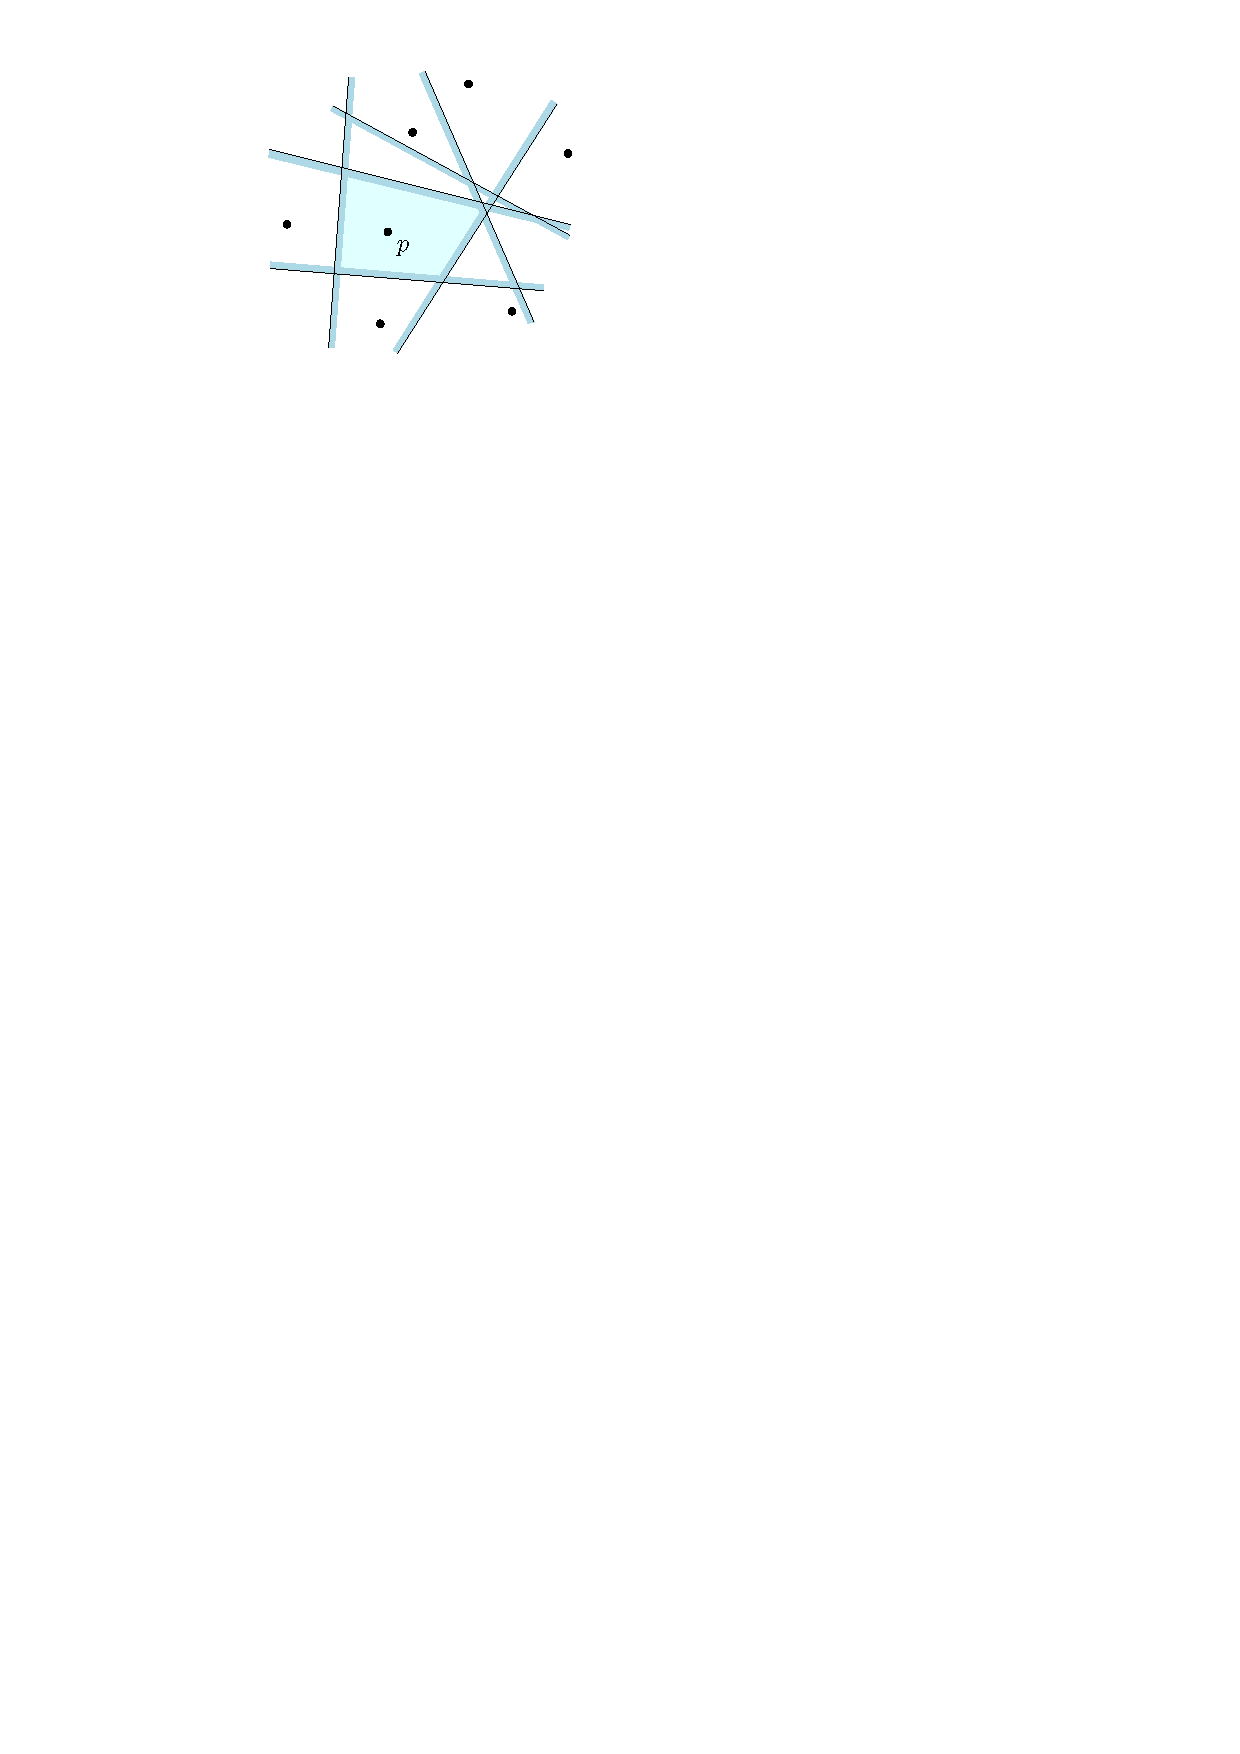
\includegraphics[width=\textwidth]{figs/halfspaces}
  \caption{The Voronoi cell $\mathcal{V}_p$ is formed by the intersection of all the half-planes between $p$ and the other points. }% 
\label{fig:halfspaces}
\end{marginfigure}
when $S$ contains more than two points (let us say it contains $n$ points), the Voronoi cell of a given point $p \in S$ is obtained by the intersection of $n-1$ half-planes defined by $p$ and the other points $q \in S$. 
That means that $\mathcal{V}_{p}$ is always convex. 
Notice also that every point $x \in \mathbb{R}^2$ has at least one nearest point in $S$, which means that VD($S$) covers the entire space.

%

As shown in Figure~\ref{fig:vd_circle}, 
\begin{marginfigure}
  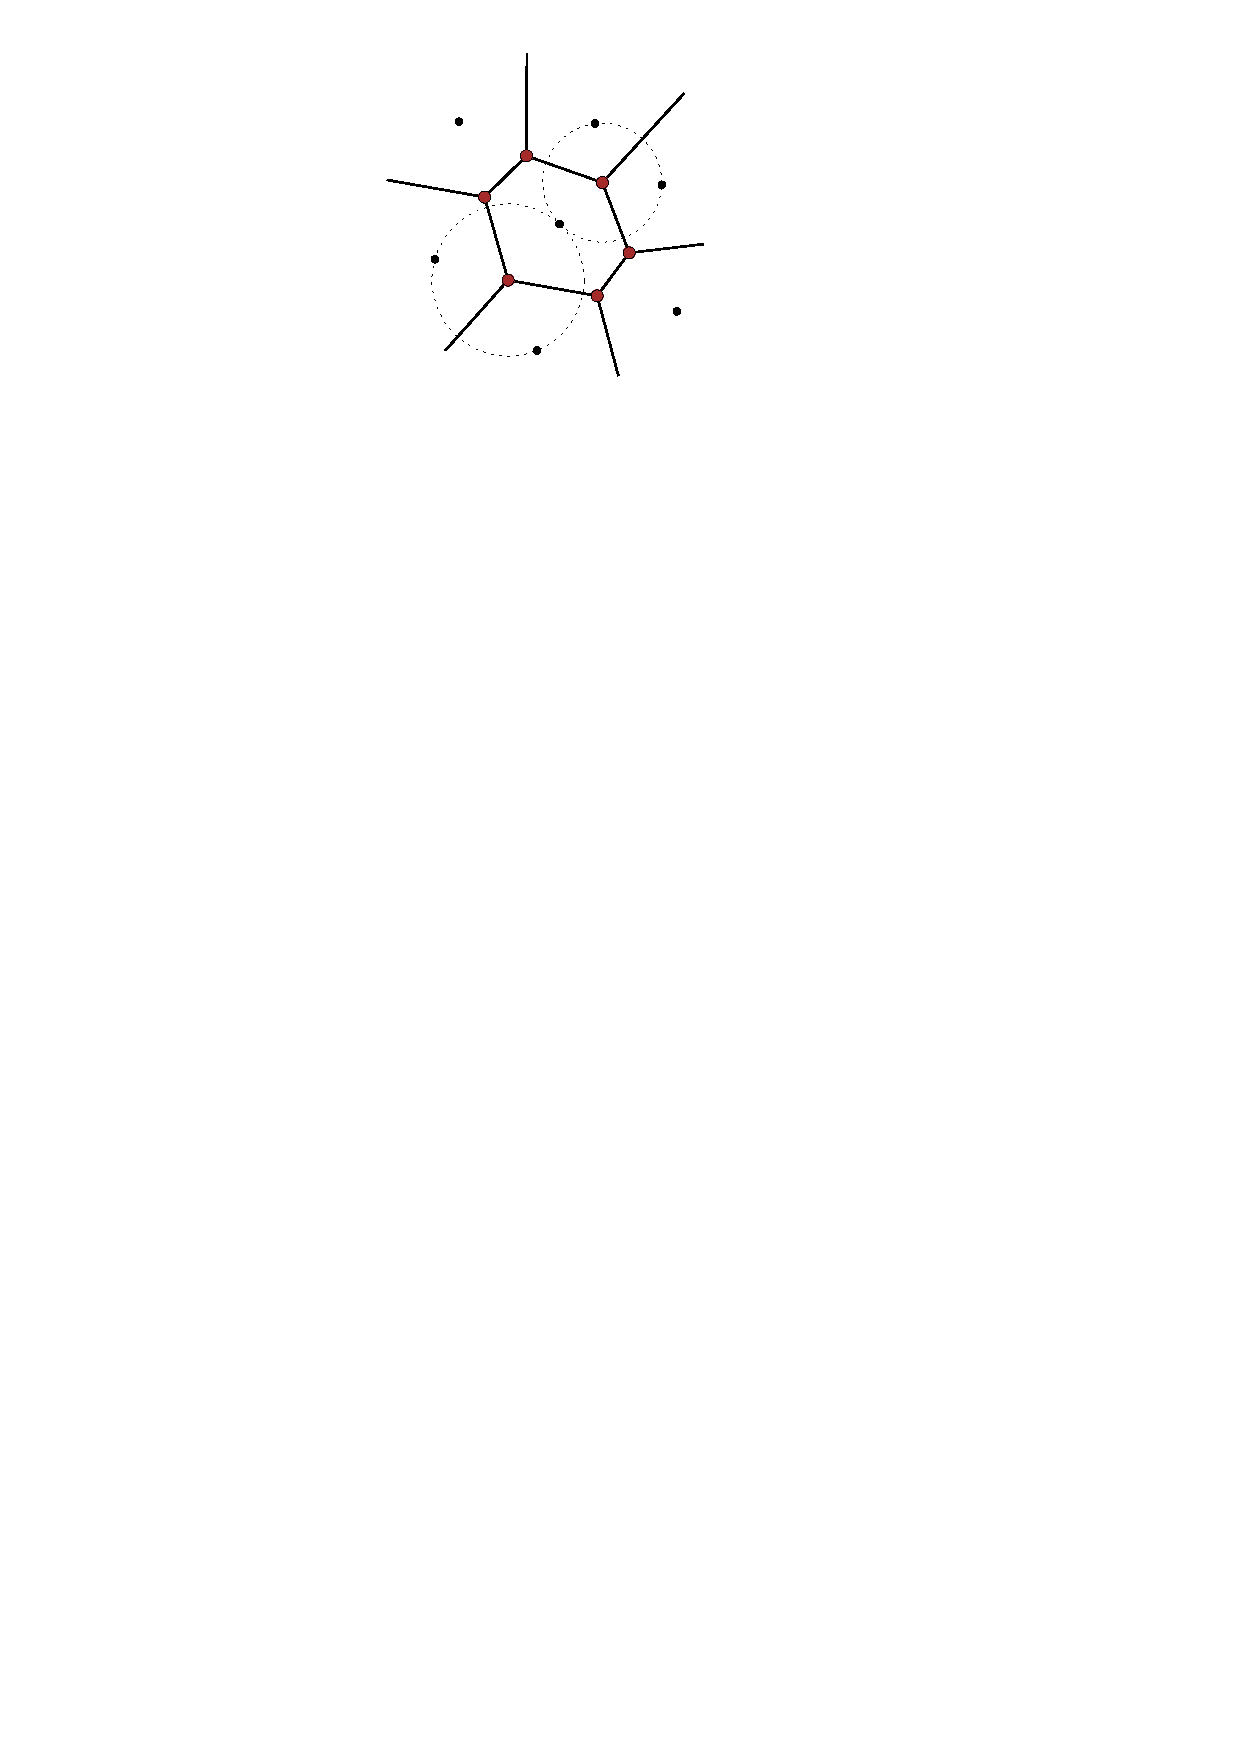
\includegraphics[width=\textwidth]{figs/vd_circle}
  \caption{The VD for a set $S$ of points in the plane (the black points). The Voronoi vertices (brown points) are located at the centre of the circle passing through three points in $S$, provided that this circle contains no other points in $S$ in its interior.}% 
\label{fig:vd_circle}
\end{marginfigure}
the VD of a set $S$ of points in $\mathbb{R}^2$ is a planar graph. 
Its edges are the perpendicular bisectors of the line segments of pairs of points in $S$, and its vertices are located at the centres of the circles passing through three points in $S$. 
The VD in $\mathbb{R}^2$ can also be seen as a two-dimensional cell complex where each 2-cell is a (convex) polygon (see Figure~\ref{fig:vd2d}). 
\begin{figure}
  \centering
  \includegraphics[page=3,width=\textwidth]{figs/vd2d}
  \caption{VD of a set of points in the plane (clipped by a box). The point $p$ (whose Voronoi cell is dark grey) has seven neighbouring cells (light grey).}% 
\label{fig:vd2d}
\end{figure}
Two Voronoi cells, $\mathcal{V}_{p}$ and $\mathcal{V}_{q}$, lie on the opposite sides of the perpendicular bisector separating the points $p$ and $q$. 

%

The VD has many interesting properties, what follows is a list of the most relevant properties in the context of this course.
\begin{description}
  \item[Size:] if $S$ has $n$ points, then VD($S$) has exactly $n$ Voronoi cells since there is a one-to-one mapping between the points and the cells.
  \item[Voronoi vertices:] a Voronoi vertex is equidistant from 3 data points. Observe for instance in Figure~\ref{fig:vd_circle} that the Voronoi vertices are at the centre of circles.
  \item[Voronoi edges:] a Voronoi edge is equidistant from 2 points.
  \item[Convex hull:] let $S$ be a set of points in $\mathbb{R}^2$, and $p$ one of its points. $\mathcal{V}_{p}$ is unbounded if $p$ bounds conv($S$). Otherwise, $\mathcal{V}_{p}$ is the convex hull of its Voronoi vertices. Observe that in Figure~\ref{fig:vd_circle}, only the point in the middle has a bounded Voronoi cell.
\end{description}
  

%%%
%
\section{Delaunay triangulation}%
\label{sec:dt_definition}\index{Delaunay triangulation}

Let $\mathcal{D}$ be the VD of a set $S$ of points in $\mathbb{R}^2$. 
Since VD($S$) is a planar graph, it has a dual graph, and let $\mathcal{T}$ be this dual graph obtained by drawing straight edges between two points $p,q \in S$ if and only if $\mathcal{V}_{p}$ and $\mathcal{V}_{q}$ are adjacent in $\mathcal{D}$. 
Because the vertices in $\mathcal{D}$ are of degree 3 (3 edges connected to it), the graph $\mathcal{T}$ is a triangulation. 
$\mathcal{T}$ is actually called the Delaunay triangulation (DT) of $S$, and, as shown in Figure~\ref{fig:dt2da}, 
\begin{figure}
  \centering
   \includegraphics[page=4,width=\textwidth]{figs/vd2d}
  \caption{The DT of a set of points in the plane (same point set as Figure~\ref{fig:vd2d}). The green circles show 2 examples of empty circumcircles.}%
\label{fig:dt2da}
\end{figure}
partitions the plane into triangles---where the vertices of the triangles are the points in $S$ generating each Voronoi cell---that satisfy the \emph{empty circumcircle} test (a circle is said to be \emph{empty} when no points are in its interior). 
If $S$ is in general position, then DT($S$) is unique.

%
\subsection{Convex hull}%
\label{sec:convexhull}\index{convex hull}

The DT of a set $S$ of points subdivides completely conv($S$), \ie\ the union of all the triangles in DT($S$) is conv($S$).

Let $S$ be a set of points in $\mathbb{R}^2$, the \emph{convex hull} of $S$, denoted conv($S$), is the minimal convex set containing $S$. 
It is best understood with the elastic band analogy: imagine each point in $\mathbb{R}^2$ being a nail sticking out of the plane, and a rubber band stretched to contain all the nails, as shown in Figure~\ref{fig:convex_hull}. 
\begin{marginfigure}
  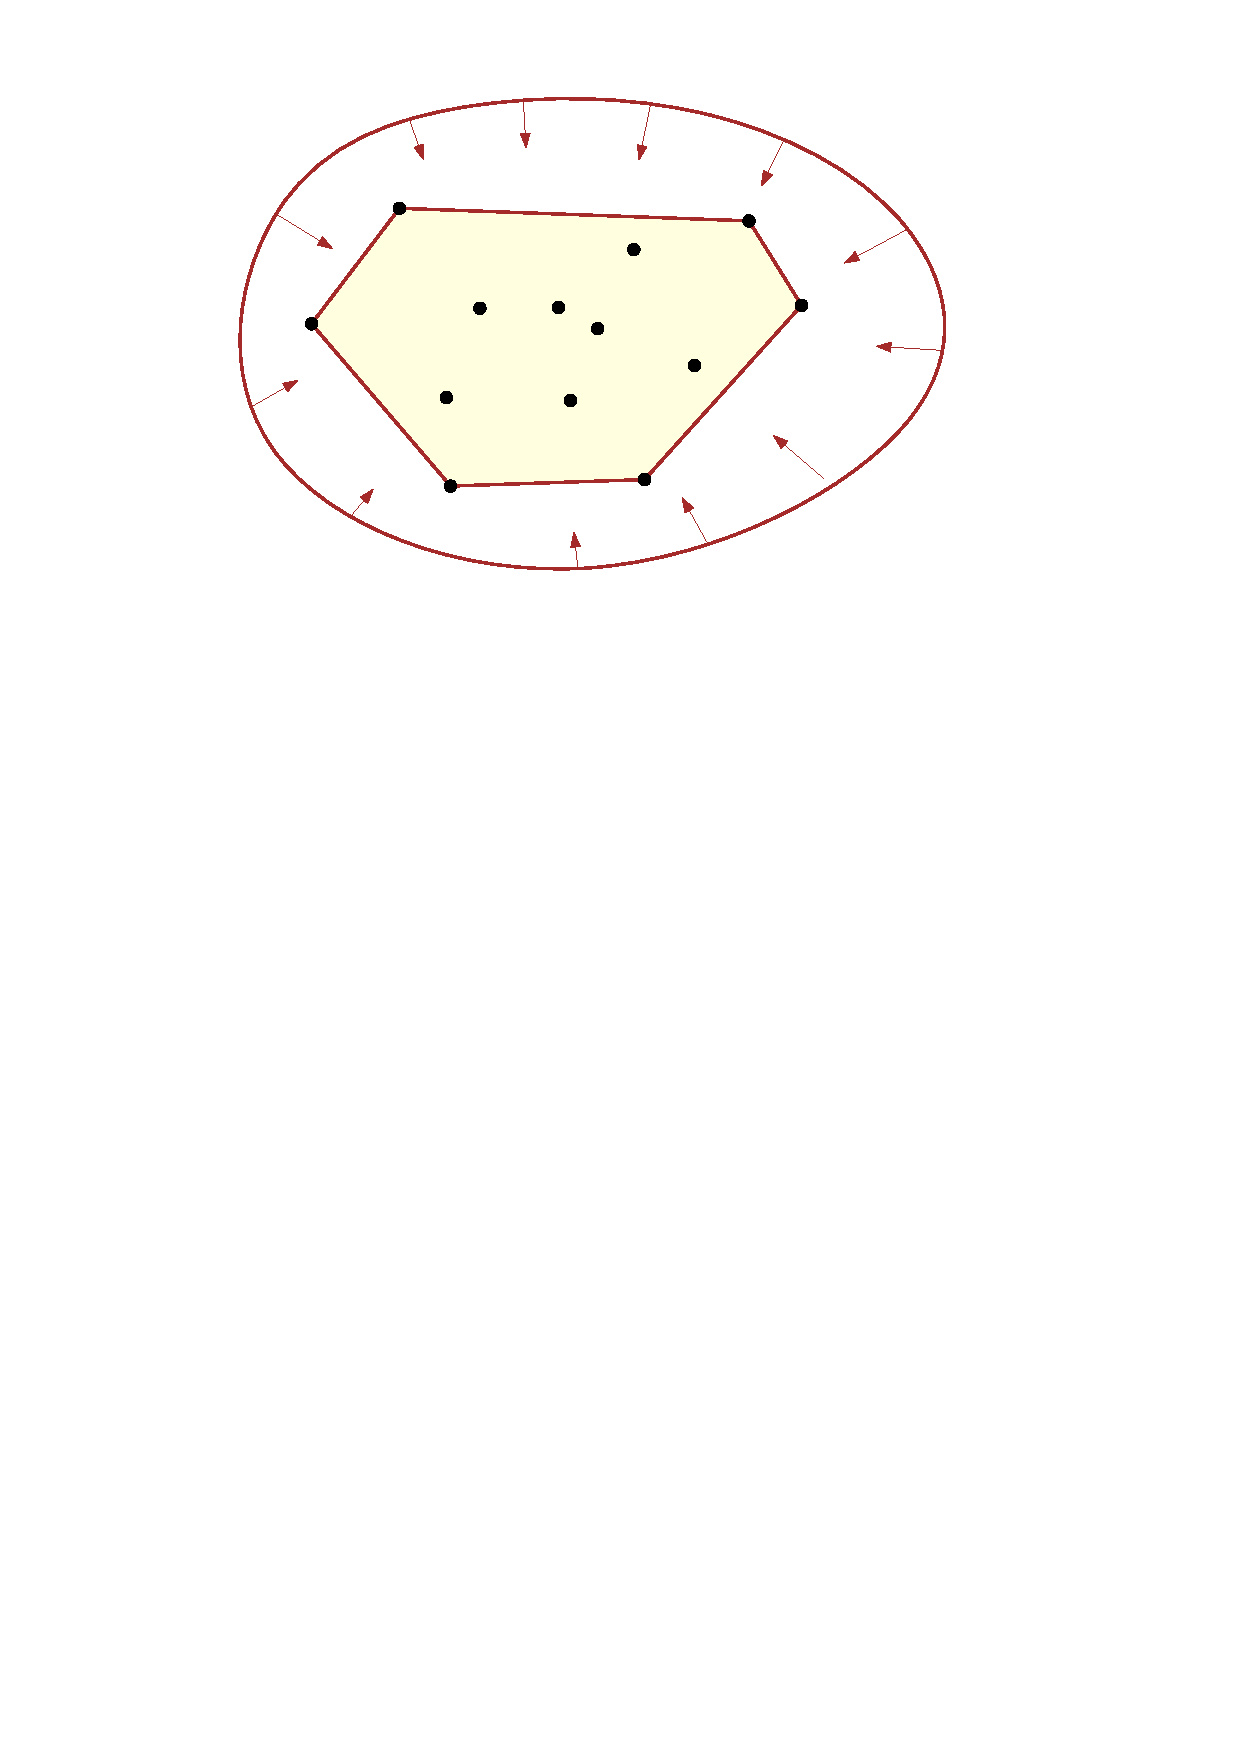
\includegraphics[width=\textwidth]{figs/convex_hull}
  \caption{The convex hull of a set of points in $\mathbb{R}^2$.}% 
\label{fig:convex_hull}
\end{marginfigure}
When released, the rubber band will assume the shape of the convex hull of the nails. 
Notice that conv($S$) is not only formed by the edges connecting the points (the rubber band), but all the points of $\mathbb{R}^2$ that are contained within these edges (thus the whole polygon).


%
\subsection{Local optimality}
Let $\mathcal{T}$ be a triangulation of $S$ in $\mathbb{R}^2$. 
An edge $\sigma$ is said to be \emph{locally} Delaunay if it either:
\begin{description}
  \item[(i)] belongs to only one triangle, and thus bounds conv($S$), or
  \item[(ii)] belongs to two triangles $\tau_a$ and $\tau_b$, formed by the vertices of $\sigma$ and respectively the vertices $p$ and $q$, and $q$ is outside of the circumcircle of $\tau_a$ (see Figure~\ref{fig:local}). 
\end{description}
Figure~\ref{fig:local} gives an example that violates the second criteria: both $p$ and $q$ are contained by the circumcircles of their opposing triangles, \ie\ of $\tau_b$ and $\tau_a$ respectively.

\begin{marginfigure}
  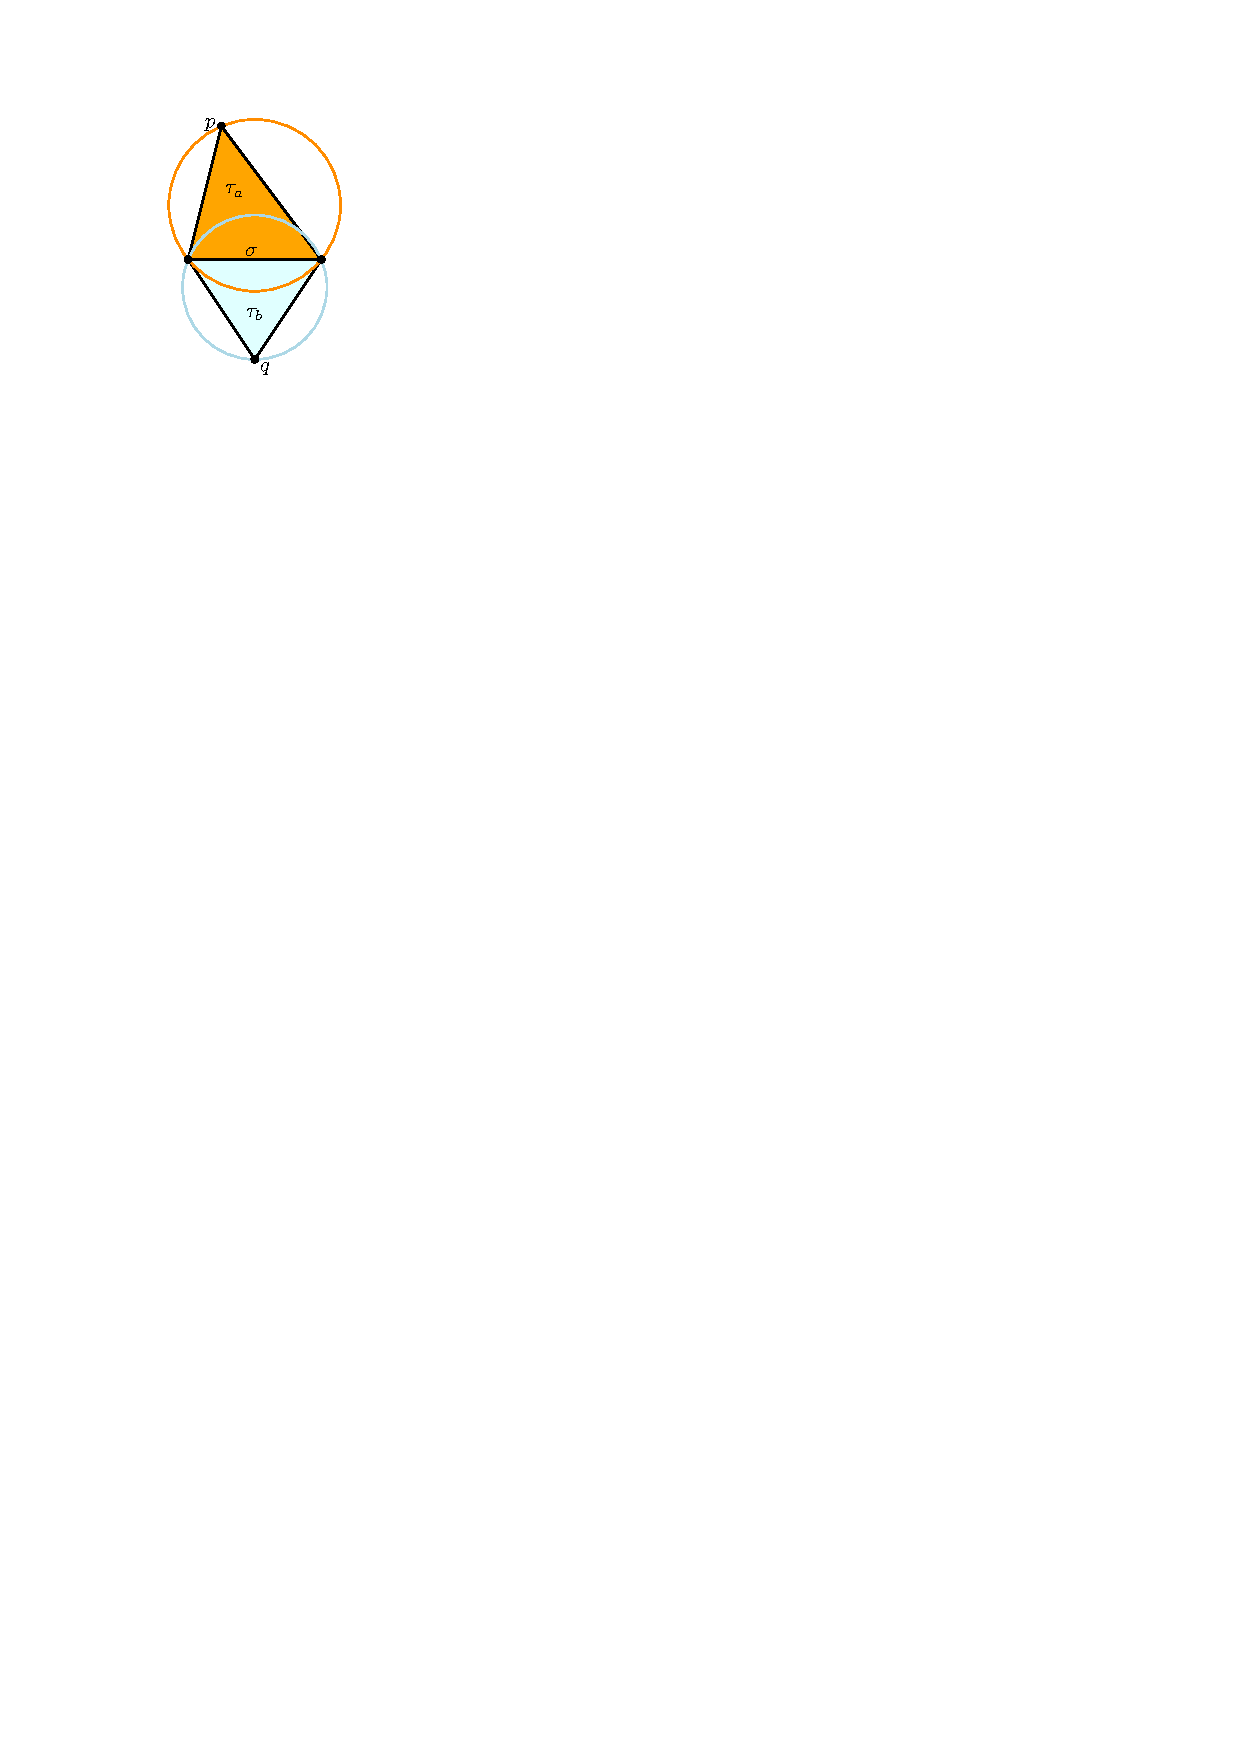
\includegraphics[width=\textwidth,page=1]{figs/local}
  \includegraphics[width=\textwidth,page=2]{figs/local}
  \caption{A quadrilateral that can be triangulated in two different ways. Only the top configuation is Delaunay. \textbf{(top)} $\sigma$ is not locally Delaunay. \textbf{(bottom)} $\sigma$ is not locally Delaunay.}%
\label{fig:local}
\end{marginfigure}

In an arbitrary triangulation, not every edge that is locally Delaunay is necessarily an edge of DT($S$), but local optimality implies globally optimality in the case of the DT:
\begin{quote}
  Let $\mathcal{T}$ be a triangulation of a point set $S$ in $\mathbb{R}^2$. If every edge of $\mathcal{T}$ is locally Delaunay, then $\mathcal{T}$ is the Delaunay triangulation of $S$.
\end{quote}
This has serious implications as the DT---and its dual---are locally modifiable, \ie\ we can theoretically insert, delete or move a point in $S$ without recomputing DT($S$) from scratch.


%%%
%
\subsection{Angle optimality}
The DT in two dimensions has a very important property that is useful in applications such as finite element meshing or interpolation: the \emph{max-min angle optimality}. Among all the possible triangulations of a set $S$ of points in $\mathbb{R}^2$, DT($S$) maximises the minimum angle (max-min property), and also minimises the maximum circumradii. 
In other words, it creates triangles that are as equilateral as possible. 
Notice here that maximising the minimum angle is not the same as minimising the maximum, and the DT only guarantees the former.


%%%
\subsection{Lifting on the paraboloid}%
\label{sec:parabolic_lifting}

There exists a close relationship between DTs in $\mathbb{R}^{2}$ and convex polyhedra in $\mathbb{R}^{3}$. 

Let $S$ be a set of points in $\mathbb{R}^{2}$. 
The parabolic lifting map projects each vertex $v(v_{x}, v_{y})$ to a vertex $v^{+}(v_{x}, v_{y}, v_{x}^{2}+v_{y}^{2})$ on the paraboloid of revolution in $\mathbb{R}^{3}$. 
The set of points thus obtained is denoted $S^{+}$. 
Observe that the paraboloid in three dimensions defines a surface whose vertical cross sections are parabolas, and whose horizontal cross sections are circles. 

%

The relationship is the following: every triangle of the lower envelope of conv($S^{+}$) projects to a triangle of the Delaunay triangulation of $S$; this is illustrated in Figure~\ref{fig:paraboloid} for a simple DT\@. 
\begin{marginfigure}
  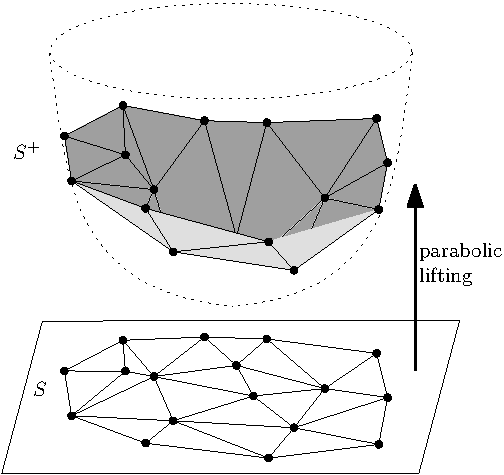
\includegraphics[width=\textwidth]{figs/paraboloid}
  \caption{The parabolic lifting map for a set $S$ of points $\mathbb{R}^2$.}%
\label{fig:paraboloid}
\end{marginfigure}

%

 Construction of the two-dimensional DT can be transformed into the construction of the convex hull of the lifted set of points in three dimensions (followed by a simple project to the two-dimensional plane).

\begin{kaobox}[frametitle=\faCog\ How does it work in practice?]
  Since it is easier to construct convex hulls (especially in higher dimensions, \ie\ 4+), the DT is often constructed with this approach, even in 2D. One popular and widely used implementation is Qhull (\url{http://www.qhull.org/}).
\end{kaobox}


%%%
%
\subsection{Degeneracies}%
\label{sec:degeneracies}

The previous definitions of the VD and the DT assumed that the set $S$ of points is in general position, \ie\ the distribution of points does not create any ambiguity in the two structures. 
For the VD/DT in $\mathbb{R}^{2}$, the degeneracies, or special cases, occur when 3 points lie on the same line and/or when 4 points are cocircular. 
For example, in two dimensions, when four or more points in $S$ are cocircular there is an ambiguity in the definition of DT($S$). 
As shown in Figure~\ref{fig:degeneracies},
\begin{marginfigure}
  \centering
  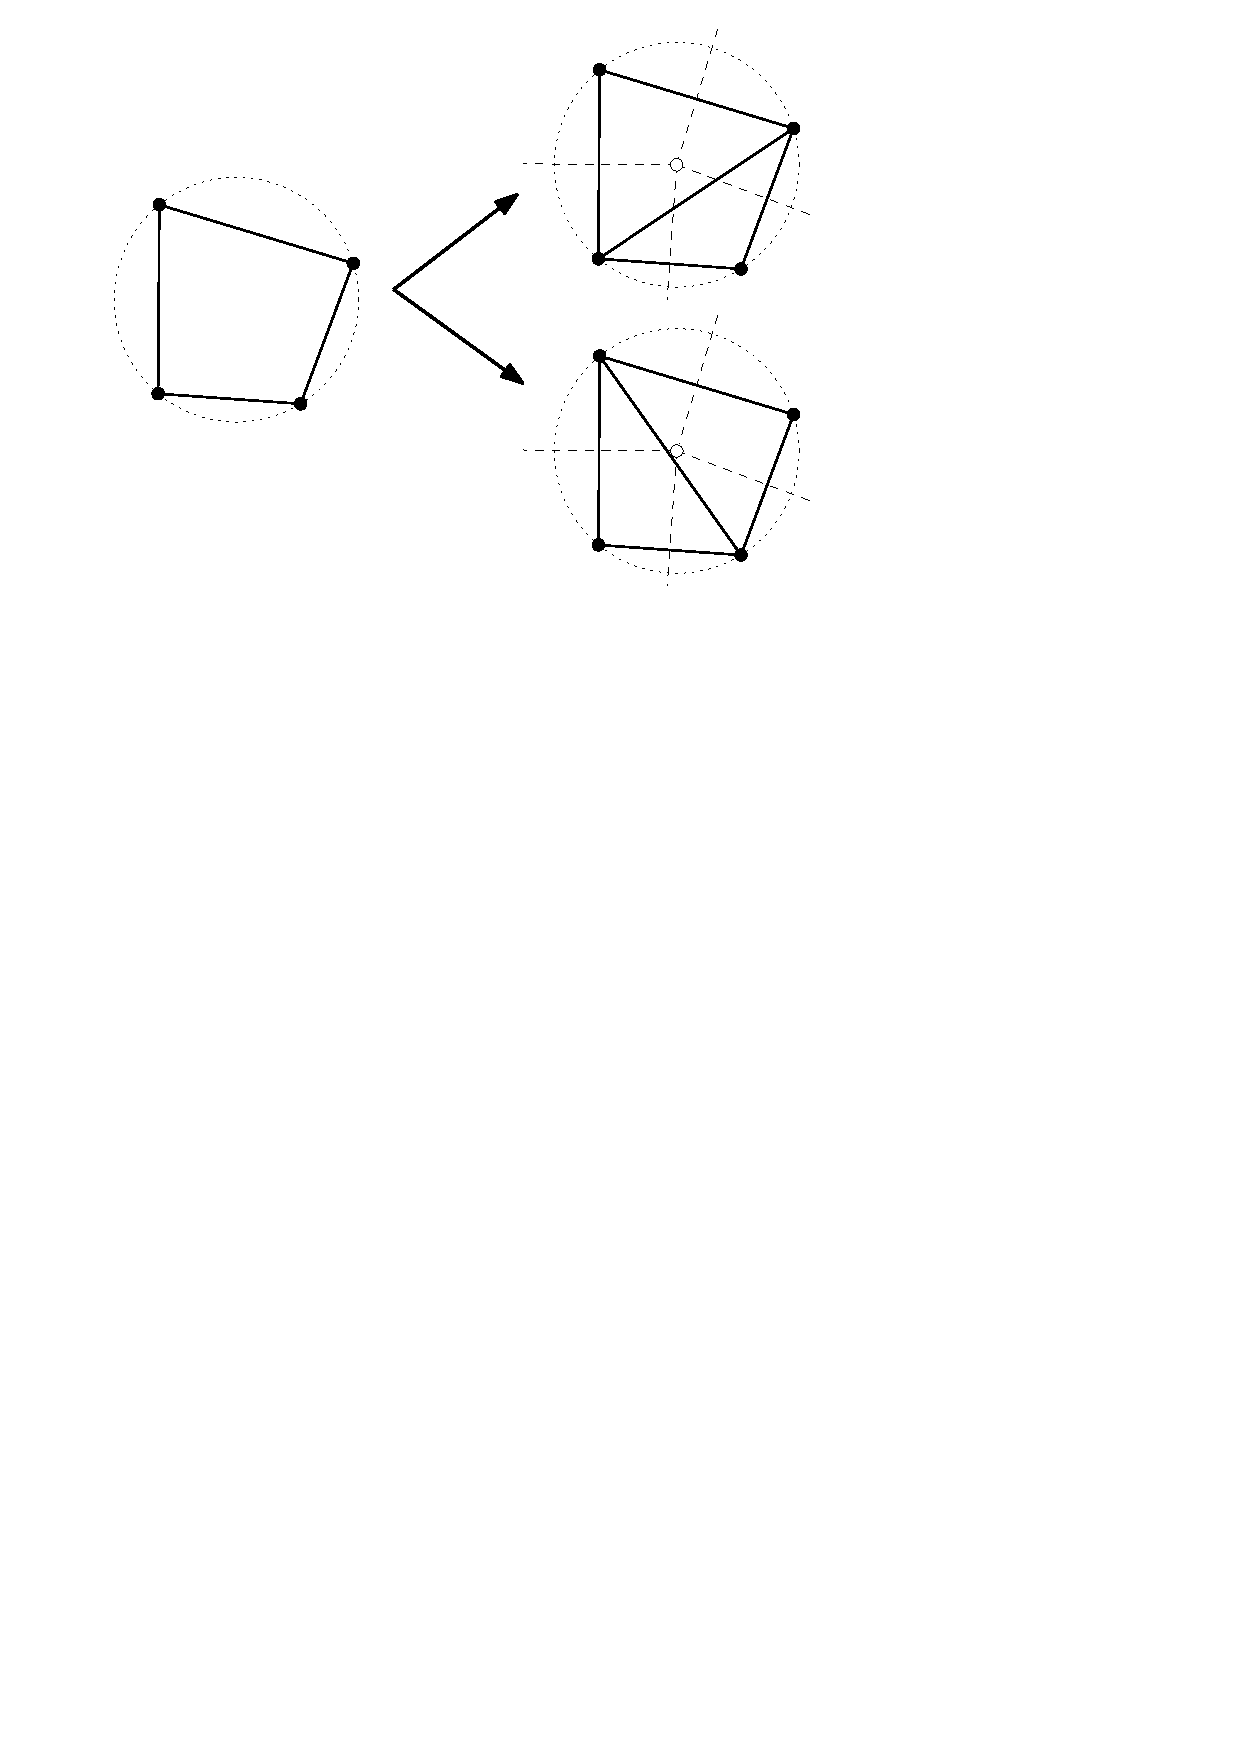
\includegraphics[width=\textwidth]{figs/degeneracies}
  \caption{The DT for four cocircular points in two dimensions is not unique (but the VD is).}%
\label{fig:degeneracies}
\end{marginfigure}
the quadrilateral can be triangulated with two different diagonals, and an arbitrary choice must be made since both respect the Delaunay criterion (points should not be on the interior of a circumcircle, but more than three can lie directly on the circumcircle).

This implies that in the presence of four or more cocircular points, DT($S$) is not unique. 
Notice that even in the presence of cocircular points, VD($S$) is still unique, but it has different properties. 
For example, in Figure~\ref{fig:degeneracies}, the Voronoi vertex in the middle has degree 4 (remember that when $S$ is in general position, every vertex in VD($S$) has degree 3). 
When three or more points are collinear, DT($S$) and VD($S$) are unique, but problems with the implementation of the structures can arise.


%%%
%
\section[Duality DT/VD]{Duality between the DT and the VD}%
\label{sec:duality}\index{duality}

Duality can have many different meanings in mathematics, but it always refers to the translation or mapping in a one-to-one fashion of concepts or structures. 
We use it in this course in the sense of the dual graph of a given graph. 
Let $G$ be a planar graph, as illustrated in Figure~\ref{fig:dual_graph} (black edges).
\begin{marginfigure}
  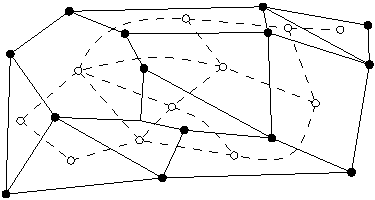
\includegraphics[width=\textwidth]{figs/dual_graph}
  \caption{A graph $G$ (black lines), and its dual graph $G^\star$ (dashed lines).}%
\label{fig:dual_graph}
\end{marginfigure}
Observe that $G$ can also be seen as a cell complex in $\mathbb{R}^{2}$. 
The duality mapping is as follows (also shown in details in Figure~\ref{fig:dualdetailtab})
The dual graph $G^{\star}$ has a vertex for each face (polygon) in $G$, and the vertices in $G^{\star}$ are linked by an edge if and only if the two corresponding dual faces in $G$ are adjacent (in Figure~\ref{fig:dual_graph}, $G^{\star}$ is represented with dashed lines). 
Notice also that each polygon in $G^{\star}$ corresponds to a vertex in $G$, and that each edge of $G$ is actually dual to one edge (an arc in Figure~\ref{fig:dual_graph}) of $G^{\star}$ (for the sake of simplicity the dual edges to the edges on the boundary of $G$ are not drawn).

The VD and the DT are the best example of the duality between plane graphs.

\begin{figure}
% \centering
% \setcapindent{1em}
\centering
\begin{minipage}[c]{0.4\textwidth}
  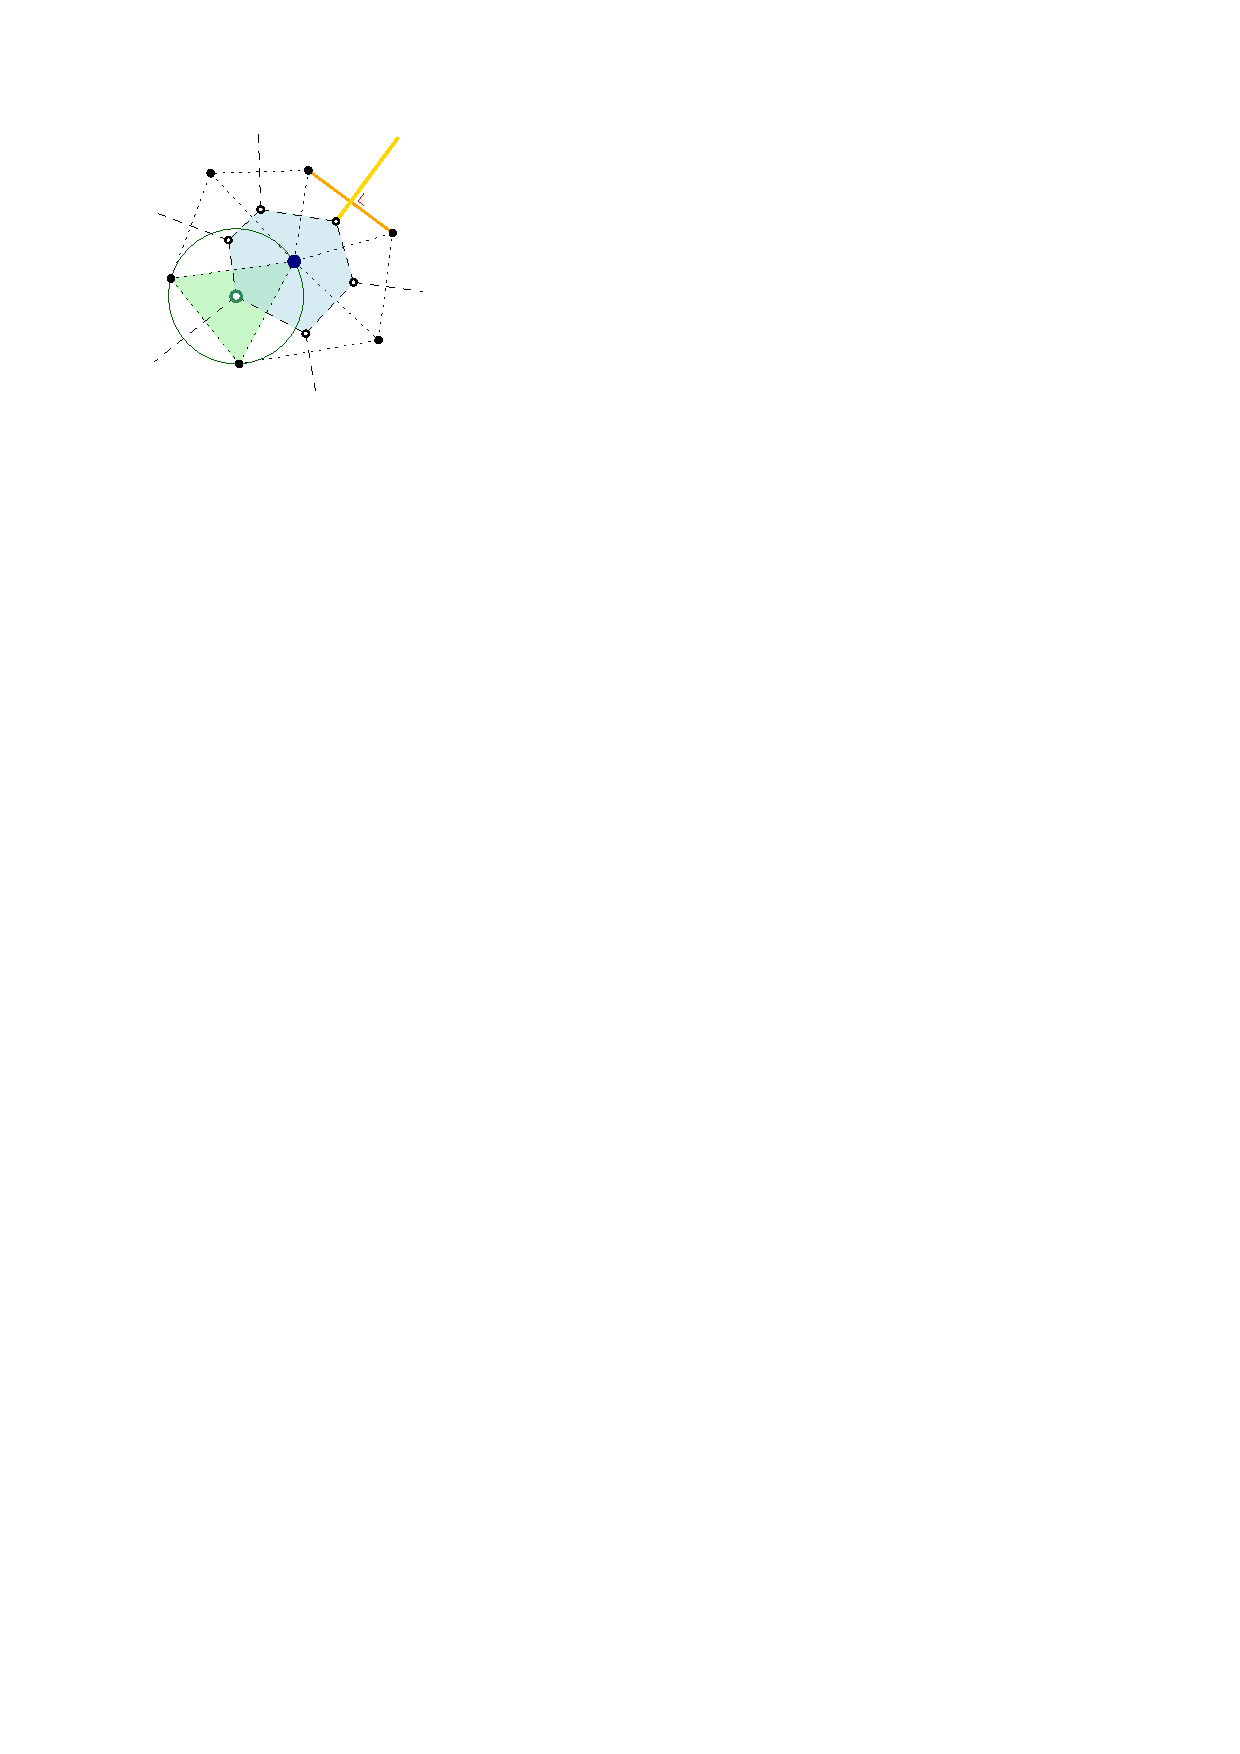
\includegraphics[width=\textwidth]{figs/dualdetail.pdf}
\end{minipage}
\begin{minipage}[c]{0.45\textwidth}
% \hspace{1.1em}
  \centering
  \begin{tabular}{lcl}
  \toprule
  DT & & VD \\
  \midrule
  $\mathbf{\color{YellowGreen}{face}}$ & $\leftrightarrow$ & $\mathbf{\color{ForestGreen}{vertex}}$\\
  $\mathbf{\color{Blue}{vertex}}$ & $\leftrightarrow$ & $\mathbf{\color{SkyBlue}{face}}$\\
  $\mathbf{\color{Orange}{edge}}$ & $\leftrightarrow$ & $\mathbf{\color{Dandelion}{edge}}$\\
  \bottomrule
  \end{tabular}
\end{minipage}
\caption{Duality between the DT (dotted) and the VD (dashed).}%
\label{fig:dualdetailtab}
\end{figure}


%%%
%
\section[DT incremental construction]{Incremental construction of the DT}%
\label{sec:dtconstruction}

Since the VD and the DT are dual structures, the knowledge of one implies the knowledge of the other one. 
In other words, if one has only one structure, she can always extract the other one. 
Because it is easier, from an algorithmic and data structure point of view, to manage triangles over arbitrary polygons (they have a constant number of vertices and neighbours), constructing and manipulating a VD by working only on its dual structure is simpler and usually preferred. 
When the VD is needed, it is extracted from the DT\@. 
This has the additional advantage of speeding up algorithms because when the VD is used directly intermediate Voronoi vertices---that will not necessarily exist in the final diagram---need to be computed and stored.

%

While there exists different strategies to construct at DT, we focus in this book on the \emph{incremental} method since it is easier to understand and implement.
An incremental algorithm is one where the structure is built incrementally; in our case this means that each point is inserted one at a time in a valid DT and the triangulation is updated, with respect to the Delaunay criterion (empty circumcircle), after each insertion. 
Observe that the insertion of a single point $p$ in a DT modifies only \emph{locally} the DT, \ie\ only the triangles whose circumcircle contains $p$ need to be deleted and replaced by new ones respecting the Delaunay criterion (see Figure~\ref{fig:insertion_deletion} for an example). 
\begin{marginfigure}
  \centering
  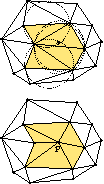
\includegraphics[width=0.9\textwidth]{figs/insertion_deletion}
  \caption{\textbf{(top)} The DT before and \textbf{(bottom)} after a point $p$ has been inserted. Notice that the DT is updated only locally (only the yellow triangles are affected).}%
\label{fig:insertion_deletion}
\end{marginfigure}

%

In sharp contrast to this, other strategies to construct a DT (\eg\ divide-and-conquer and plane sweep algorithms, see Section~\ref{sec:notes}), build a DT in \emph{one} operation (this is a batch operation), and if another point needs to be inserted after this, the whole construction operation must be done again from scratch. 
That hinders their use for some applications where new data coming from a sensor would have to be added.

%

The incremental insertion algorithm, and the other well-known algorithms, can all construct the DT of $n$ points randomly distributed in the Euclidean plane in $\mathcal{O}(n \log n)$.

%

Figure~\ref{fig:insertion_steps} illustrates the steps of the algorithm, and Algorithm~\ref{algo:insert1pt} its pseudo-code. 
\begin{figure*}
  \centering
  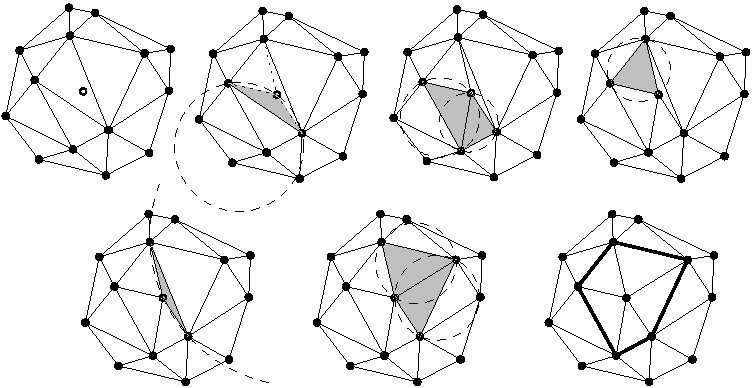
\includegraphics[width=\textwidth]{figs/insertion_steps}
  \caption{Step-by-step insertion, with flips, of a single point in a DT in two dimensions.}%
\label{fig:insertion_steps}
\end{figure*}
\begin{algorithm}[tb] 
  \DontPrintSemicolon\
  \KwIn{A DT($S$) $\mathcal{T}$, and a new point $p$ to insert}
  \KwOut{$\mathcal{T}^{p} = \mathcal{T} \cup \{p\}$ // the DT with point $p$}
  find triangle $\tau$ containing $p$\;
  insert $p$ in $\tau$ by splitting it in to 3 new triangles (flip13)\;
  push 3 new triangles on a stack\;
  \While{stack is non-empty}
  {
    $\tau = \{p,a,b\} \leftarrow$ pop from stack\;
    $\tau_{a} = \{a,b,c\} \leftarrow$ get adjacent triangle of $\tau$ having the edge $ab$\;
    \If{$c$ is inside circumcircle of $\tau$}
    {
      flip22 $\tau$ and $\tau_{a}$\;
      push 2 new triangles on stack\;
    }
  }
  \caption{Algorithm to insert one point in a DT}%
\label{algo:insert1pt}
\end{algorithm} 
In a nutshell, for the insertion of a new point $p$ in a DT($S$), the triangle $\tau$ containing $p$ is identified and then split into three new triangles by joining $p$ to every vertex of $\tau$. 
Second, each new triangle is tested---according to the Delaunay criterion---against its opposite neighbour (with respect to $p$); if it is not a Delaunay triangle then the edge shared by the two triangles is \emph{flipped} (see below) and the two new triangles will also have to be tested later. 
This process stops when every triangle having $p$ as one of its vertices respects the Delaunay criterion.


%%%
\paragraph{Initialisation: the big triangle.}%
\label{sec:big_tr}
Most of the incremental DT/VD algorithms assume that the set $S$ of points is entirely contained in a \emph{big triangle} ($\tau_{big}$) several times larger than the spatial extent of $S$; conv($S$) therefore becomes $\tau_{big}$. 
Figure~\ref{fig:big_tr} illustrates this.
\begin{marginfigure}
  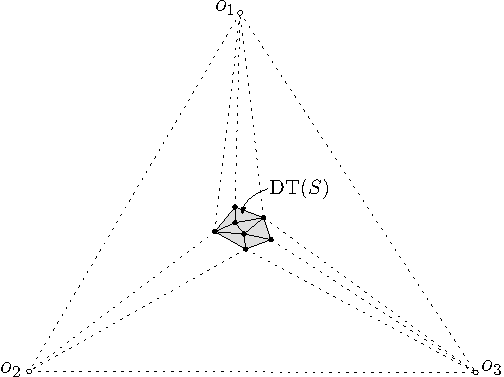
\includegraphics[width=\textwidth]{figs/big_tr}
  \caption[The big triangle containing all the dataset.]{The set $S$ of points is contained by a \emph{big triangle} formed by the vertices $o_1$, $o_2$ and $o_3$. Many triangles outside conv($S$) are created.}% 
\label{fig:big_tr}
\end{marginfigure}
The construction of DT($S$) is for example always initialised by first constructing $\tau_{big}$, and then the points in $S$ are inserted one by one. 

%

Doing this has many advantages. 
First, when a single point $p$ needs to be inserted in DT($S$), this guarantees that $p$ is always inside an existing triangle; we thus do not have to deal explicitly with vertices added outside the convex hull. 
Second, we do not have to deal with the (nasty) case of deleting a vertex that bounds conv($S$). 
Third, since an edge is always guaranteed to be shared by two triangles, point location algorithms never ``fall off'' the convex hull. 
Fourth, identifying the vertices that bounds conv($S$) is easy: they have one incident triangle that has one or more of the big triangle vertices.
Fifth, the Voronoi cells of the points that bounds conv($S$) will be bounded, since the only unbounded cells will be the ones of the four points of $\tau_{big}$. 
This can help for some of the spatial analysis operations, for instance interpolation based on the VD (see Chapter~\ref{chap:interpol}).

%

The main disadvantage is that more triangles than needed are constructed. 
For example in Figure~\ref{fig:big_tr} only the shaded triangles would be part of DT($S$). 
The extra triangles can nevertheless be easily marked as they are the only ones containing at least one of the three points forming $\tau_{big}$. 

%

\begin{kaobox}[frametitle=\faCog\ How does it work in practice?]
Several implementations of the DT use a big triangle,  CGAL (\url{https://www.cgal.org/}) being one example, and these often label vertices and/or triangles as ``infinite''.
It is therefore essential to understand the mecanism, even if one is not constructing the DT herself.
There is also a variation on the big triangle: when an extra point is ``at the infinity''.
\end{kaobox}


%%%
\paragraph{Point location with walking.}% 
\label{sec:dtwalk}

To find the triangle containing the newly inserted point $p$, we can use the point-in-polygon test for every triangle (the standard GIS operation), but that brute-force operation would be very slow (complexity would be $\mathcal{O}(n)$ since each triangle must be checked).

A better alternative is to use the adjacency relationships between the triangles, and use a series of \Orient\ tests, as described below, to navigate from one triangle to the other. 
The idea, called ``walking'', is shown in Figure~\ref{fig:walk} and details are given in the Algorithm~\ref{algo:walk}.
\begin{figure}
  \centering
  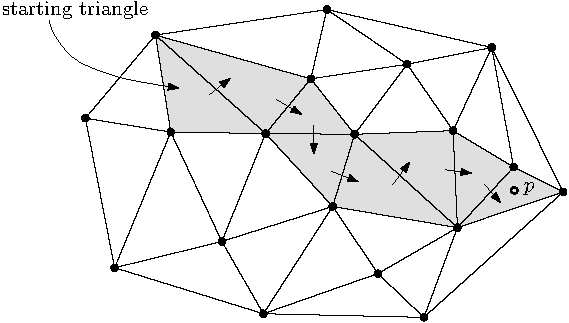
\includegraphics[width=0.7\textwidth]{figs/walk}
  \caption{The Walk algorithm for a DT in two dimensions. The query point is $p$.}%
\label{fig:walk}
\end{figure}
\begin{algorithm}[t]
  \DontPrintSemicolon\
  \KwIn{A DT($S$) $\mathcal{T}$, a starting triangle $\tau$, and a query point $p$}
  \KwOut{$\tau_r$: the triangle in $\mathcal{T}$ containing $p$}
  \BlankLine\ 
  $\tau_r$ = None\;
  \While{$\tau_r$ == None}
  {
    visitededges = 0\;
    \For{$i \leftarrow 0$ \KwTo\ 2}
    {
      $\sigma_i \leftarrow$ get edge opposite to vertex $i$ in $\tau$\;
      \If{\Orient($\sigma_i, p$) $< 0$\nllabel{l:walk}} 
      {
        $\tau \leftarrow$ get neighbouring triangle of $\tau$ incident to $\sigma_i$\;
        break\;
      }
      visitededges += 1\;
    }  
    \If{$visitededges == 3$}
    {
      \tcp{all the edges of $\tau$ have been tested}
      $\tau_r$ = $\tau$\;
    }
  }
  Return($\tau_r$)
  \caption{W\textsc{alk}($\mathcal{T}$, $\tau$, $p$)}%
\label{algo:walk}
\end{algorithm}
The idea is as follows: in a DT($S$), starting from a triangle $\tau$ (it can be any), we move to one of the adjacent triangle of $\tau$ ($\tau$ has three neighbours, we choose one neighbour $\tau_i$ such that the query point $p$ and $\tau$ are on each side of the edge shared by $\tau$ and $\tau_i$) until there is no such neighbour, then the simplex containing $p$ is the current triangle $\tau$.
Notice that this algorithm is not affected by degenerate cases, and that if an \textrm{O}\textsc{rientation} test returns 0 (collinearity), then it is simply considered a positive result. 
This will ensure that if the query point $p$ is located exactly at the same position as one point in $S$, then one triangle incident to $p$ will be returned.


%%%
\paragraph{Flips.}
The \emph{flip22} operation used to modify the triangulation is a simple \emph{local} topological operation that modifies the configuration of two adjacent triangles. 
It is performed in constant time $\mathcal{O}(1)$.
Consider the set $S = \{a, b, c, d\}$ of points in the plane forming a quadrilateral, as shown in Figure~\ref{p:flip22}. 
\begin{marginfigure}
  \centering
  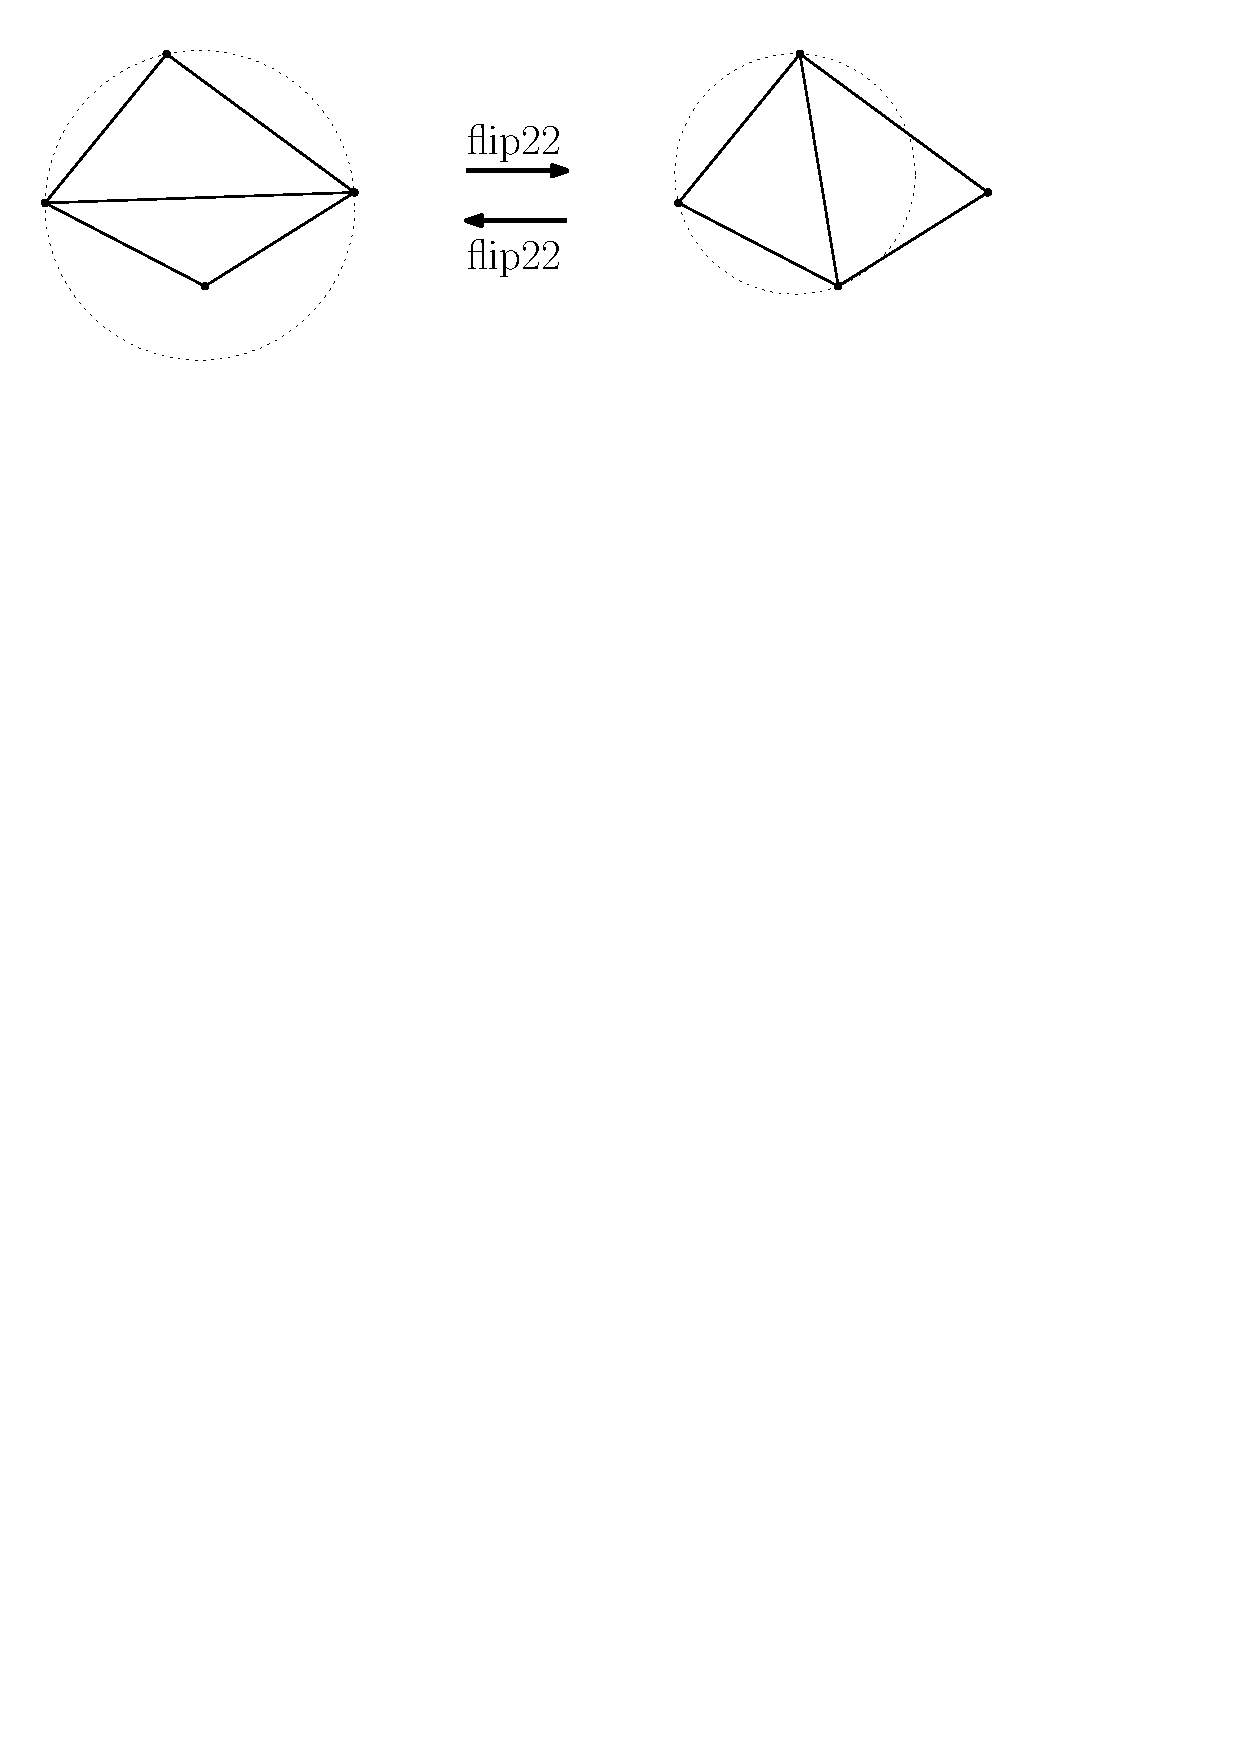
\includegraphics[width=0.5\textwidth]{figs/flip22}
  \caption{A flip22}%
\label{p:flip22}
\end{marginfigure}
There exist exactly two ways to triangulate $S$: the first one contains the triangles $abc$ and $bcd$; and the second one contains the triangles $abd$ and $acd$. 
Only the first triangulation of $S$ is Delaunay because $d$ is outside the circumcircle of $abc$. 
A \emph{flip22} is the operation that transforms the first triangulation into the second, or vice-versa.

Two other flips are possible: \emph{flip13} and \emph{flip31}; the numbers refer to the number of triangles before and after the flip.
A flip13 refers to the operation of inserting a vertex inside a triangle, and splitting it into three triangles; and a flip31 is the inverse operation that deletes a vertex.


%%%
\paragraph{Controlling the flips.}
To control which triangles have to be checked and potentially flipped, we use a stack\footnote{A data structure: \url{https://en.wikipedia.org/wiki/Stack_(abstract_data_type)}}. 
When the stack is empty, then there are no more triangles to be tested, and we are guaranteed that all the triangles in the triangulation have an empty circumcircle.


%%%
\paragraph{Predicates.}\index{predicates}
Constructing a DT and manipulating it essentially require two basic geometric tests (called \emph{predicates}): \Orient\ determines if a point $p$ is left, right or lies on the line segment defined by two points $a$ and $b$; and \Incircle\ determines if a point $p$ is inside, outside or lies on a circle defined by three points $a$, $b$ and $c$. 
Both tests can be reduced to the computation of the determinant of a matrix:
\begin{equation}
  \textrm{O}\textsc{rientation}(a, b, p) = 
  \left| 
  \begin{array}{cccc}
    a_{x} & a_{y} & 1 \\
    b_{x} & b_{y} & 1 \\
    p_{x} & p_{y} & 1 
  \end{array} 
  \right| 
\end{equation}
\begin{equation}
  \textrm{I}\textsc{n}\textrm{C}\textsc{ircle}(a, b, c, p) = 
  \left| 
  \begin{array}{ccccc}
    a_{x} & a_{y} & a^{2}_{x} + a^{2}_{y} & 1 \\
    b_{x} & b_{y} & b^{2}_{x} + b^{2}_{y} & 1 \\
    c_{x} & c_{y} & c^{2}_{x} + c^{2}_{y} & 1 \\
    p_{x} & p_{y} & p^{2}_{x} + p^{2}_{y} & 1 
  \end{array} 
  \right|%
\label{eq:insphere}
\end{equation}


%%%%%%%%%%%%%%%%%%%%%%%%%%%%
%%%%%%%%%%%%%%%%%%%%%%%%%%%%
\section[DT data structures]{Data structures for storing a DT}

A triangulation is simply a subdivision of the plane into polygons, and thus any data structure used in GIS can be used to store a triangulation.

\begin{description}
  \item[Simple Features:] while many use this (PostGIS and any triangulation you see in Shapefiles), this is not smart: (1) the topological relationships between the triangles are not stored; (2) the vertices are repeated for each triangle (and we know that for a Poisson distribution of points in the plane a given point has exactly 6 incident triangles).
  \item[Edge-based structures:] all the edge-based topological data structure used for storing planar graphs (\eg\ DCEL, half-edge, winged-edge, etc) can be used. These usually lead to large storage space.
\end{description}

Observe that in practice, if only the DT is wanted (and not the constrained one, see below), practitioners will often simply store the sample points and reconstruct on-the-fly the DT, since it is unique (if we omit points not in general position that is).

However, because it is simpler to manage triangles over arbitrary polygons (they always have exactly 3 vertices and 3 neighbours), data structures specific for triangulations have been developed and are usually used.

The simplest data structure, as shown in Figure~\ref{fig:tr_ds}, 
\begin{figure}
  \centering
  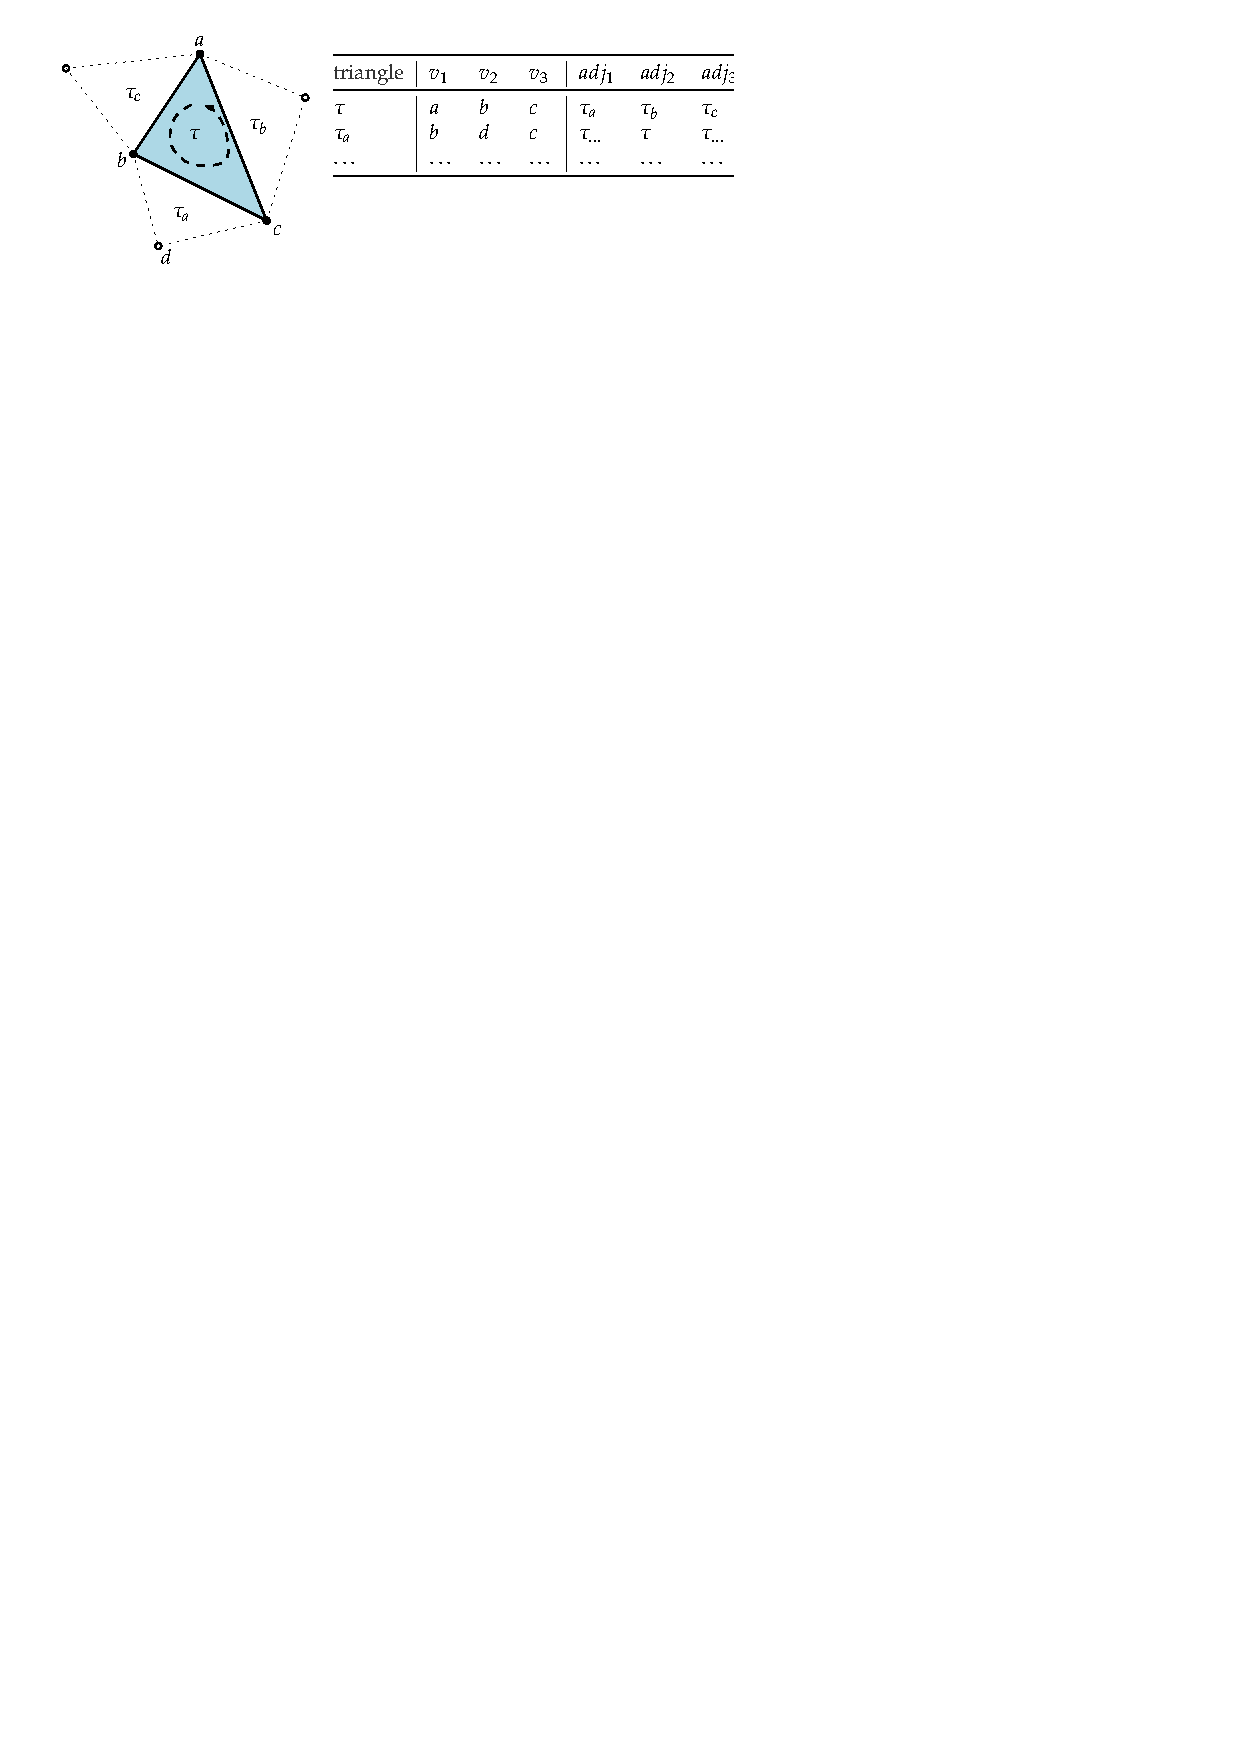
\includegraphics[width=\linewidth]{figs/tr_ds}
  \caption{The triangle-based data structure to store efficiently a triangulation (and the adjacency relationships between the triangles).}%
\label{fig:tr_ds}
\end{figure}
considers the triangle as being its atom and stores each triangle with 3 pointers to its vertices and 3 pointers to its adjacent triangles. 
Observe that the order in which the vertices and adjacent triangles stored correspond to each other. 
This is an important property that allows an efficient retrieval of triangles in the Walk algorithm (Algorithm~\ref{algo:walk}) for instance.



%%%%%%%%%%%%%%%%%%%%%%%%%%%%
\section{Constrained and Conforming Delaunay Triangulations}%
\index{Constrained DT}\index{CDT}

Given as input a set $S$ of points and straight-line segments in the plane, different triangulations of $S$ (so that the segments are respected) can be constructed. 
We are mostly interested in the \emph{constrained Delaunay triangulation} (ConsDT) and the \emph{conforming Delaunay triangulation} (ConfDT), see Figure~\ref{fig:cdt_example} for one example.
\begin{marginfigure}
  \centering
  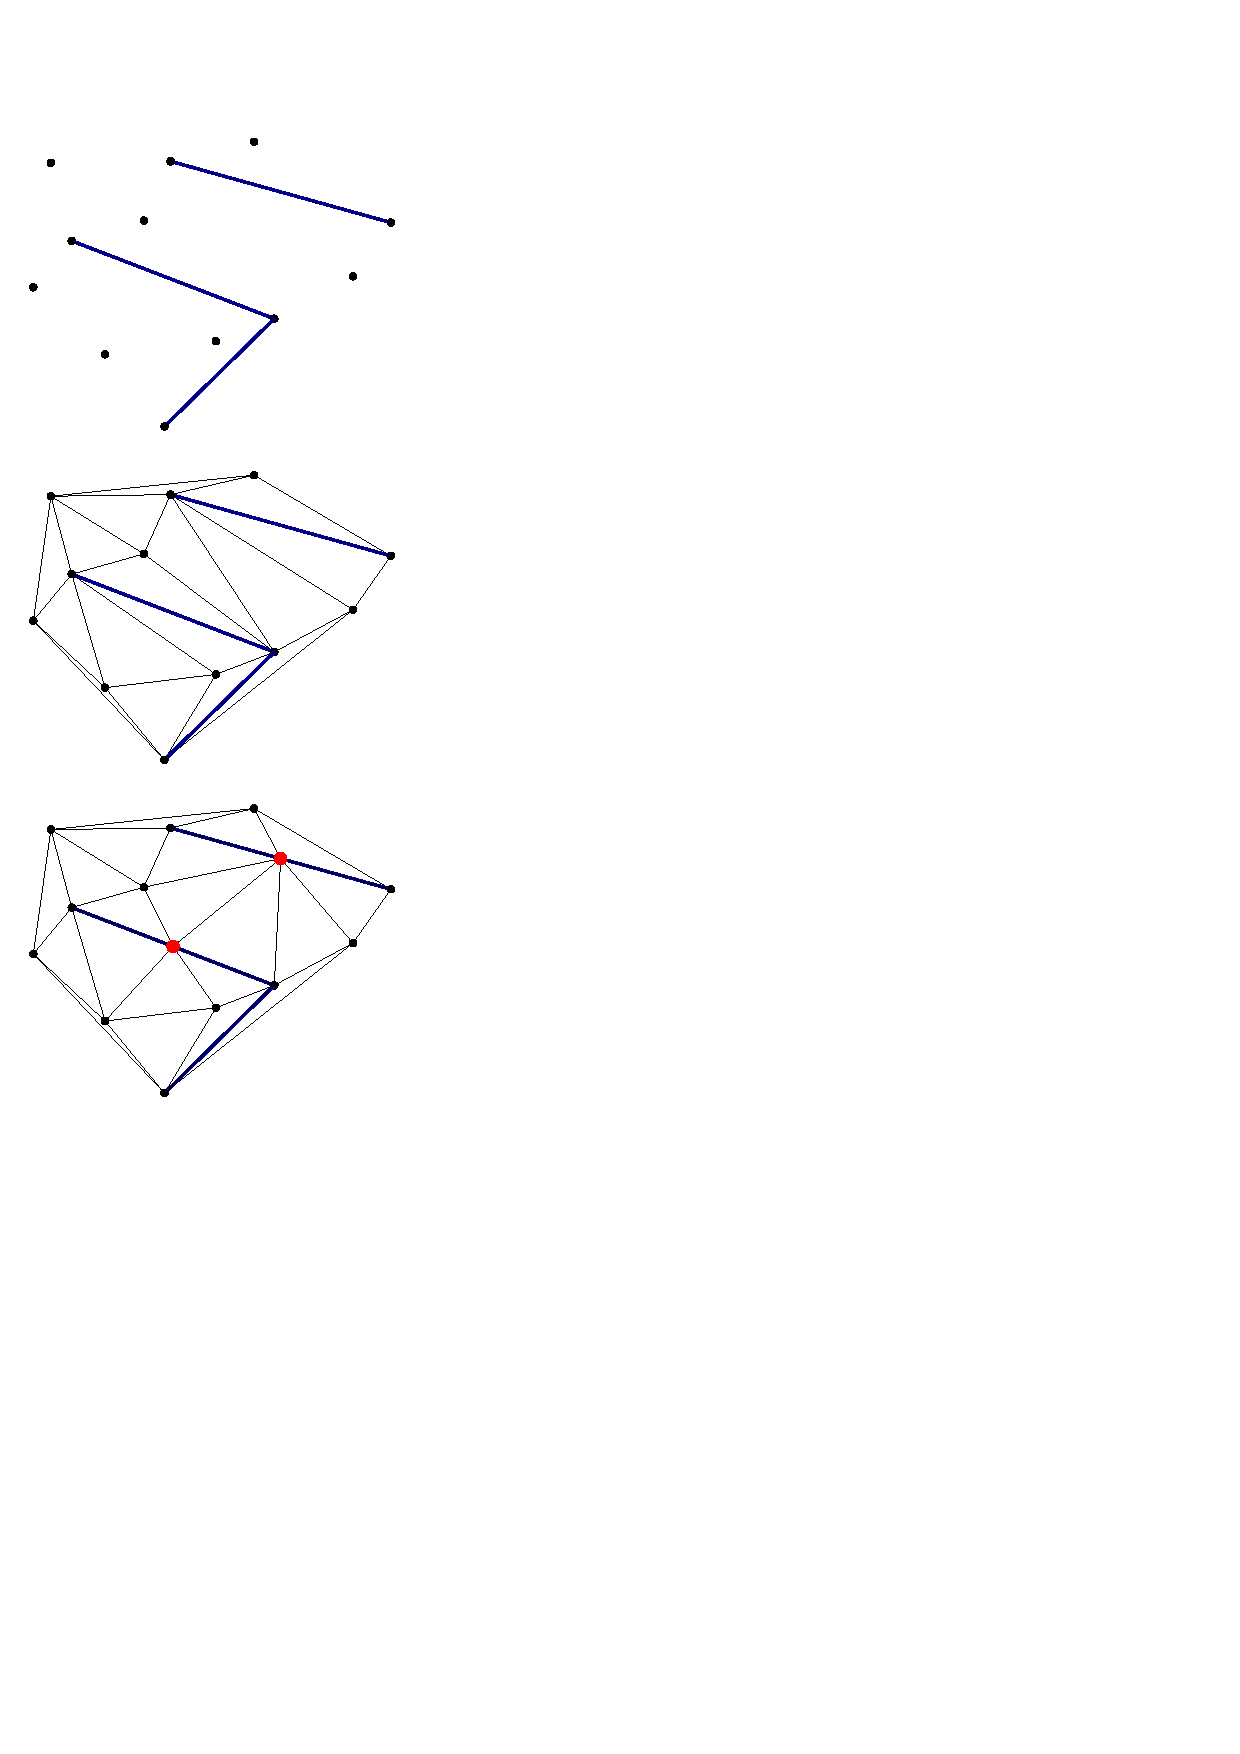
\includegraphics[width=0.85\linewidth]{figs/cdt_example}
  \caption{\textbf{(top)} A set $S$ of points and straight-line segments. \textbf{(middle)} Constrained DT of $S$. \textbf{(bottom)} Conforming DT of $S$; the Steiner points added are in red.}%
\label{fig:cdt_example}
\end{marginfigure}

%%%
%
\paragraph*{Constrained DT (ConsDT).}
Given a set $S$ of points and straight-line segments in $\mathbb{R}^2$, the ConsDT permits us to decompose the convex hull of $S$ into non-overlapping triangles, and every segment of $S$ appears as an edge in ConsDT($S$). 
ConsDT is similar to the Delaunay triangulation, but the triangles in ConsDT are not necessarily Delaunay (\ie\ their circumcircle might contain other points from $S$). 
The empty circumcircle for a ConsDT is less strict: a triangle is Delaunay if its circumcircle contains no other points in $S$ that are \emph{visible} from the triangle.
The constrained segments in $S$ act as visibility blockers. 
Figure~\ref{fig:cdt_buildings} shows one example.
\begin{figure}
  \centering
  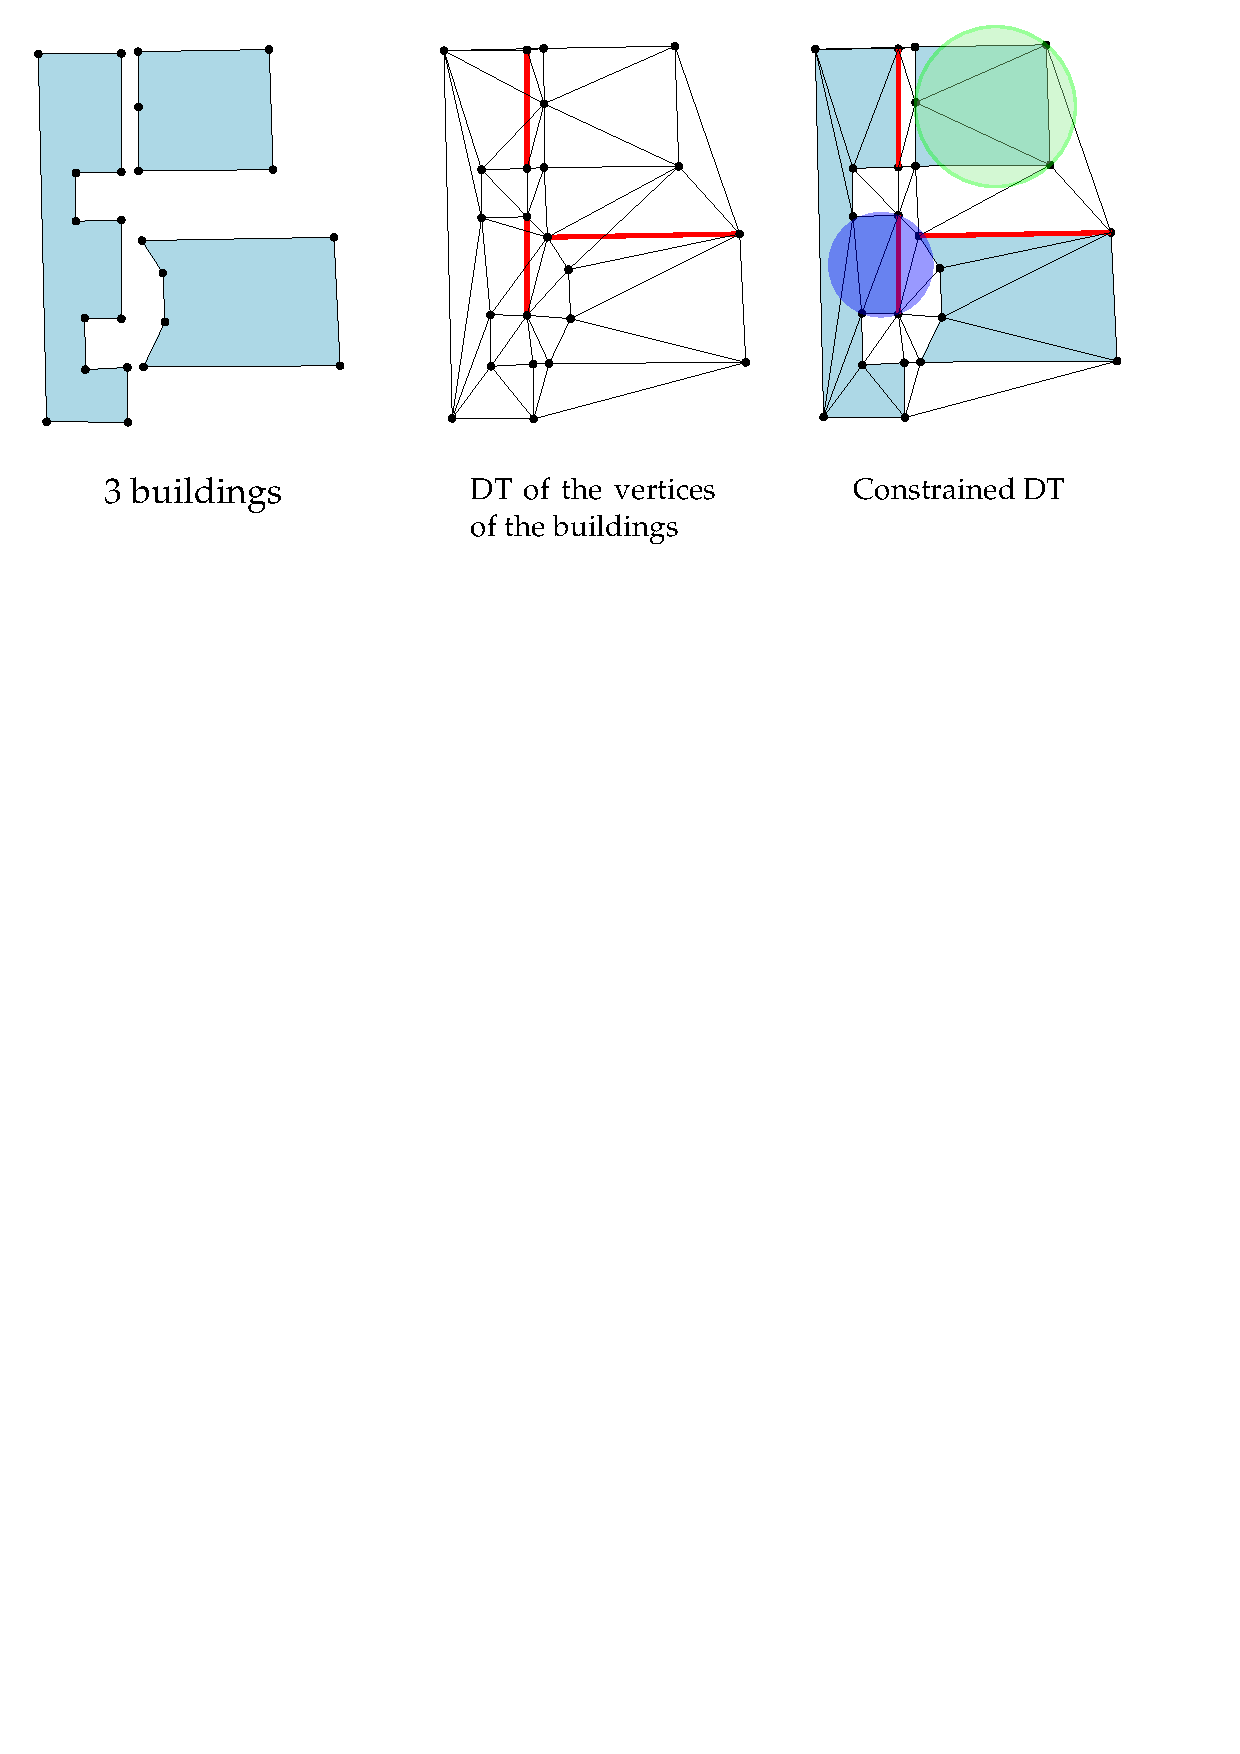
\includegraphics[width=0.95\textwidth]{figs/cdtbuildings}
  \caption{The ConsDT of a set of segments. On the right, the triangle whose circumcircle is green is a Delaunay (no other points in its interior) and so is the triangle whose circumcircle is in purple (there is one point in its interior, but it cannot be seen because of the constrained segment).}%
\label{fig:cdt_buildings}
\end{figure}

%

Without going into details about one potential algorithm, one way to construct a ConsDT($S$) is (see Figure~\ref{fig:cdt_steps}):
\begin{figure*}
  \centering
  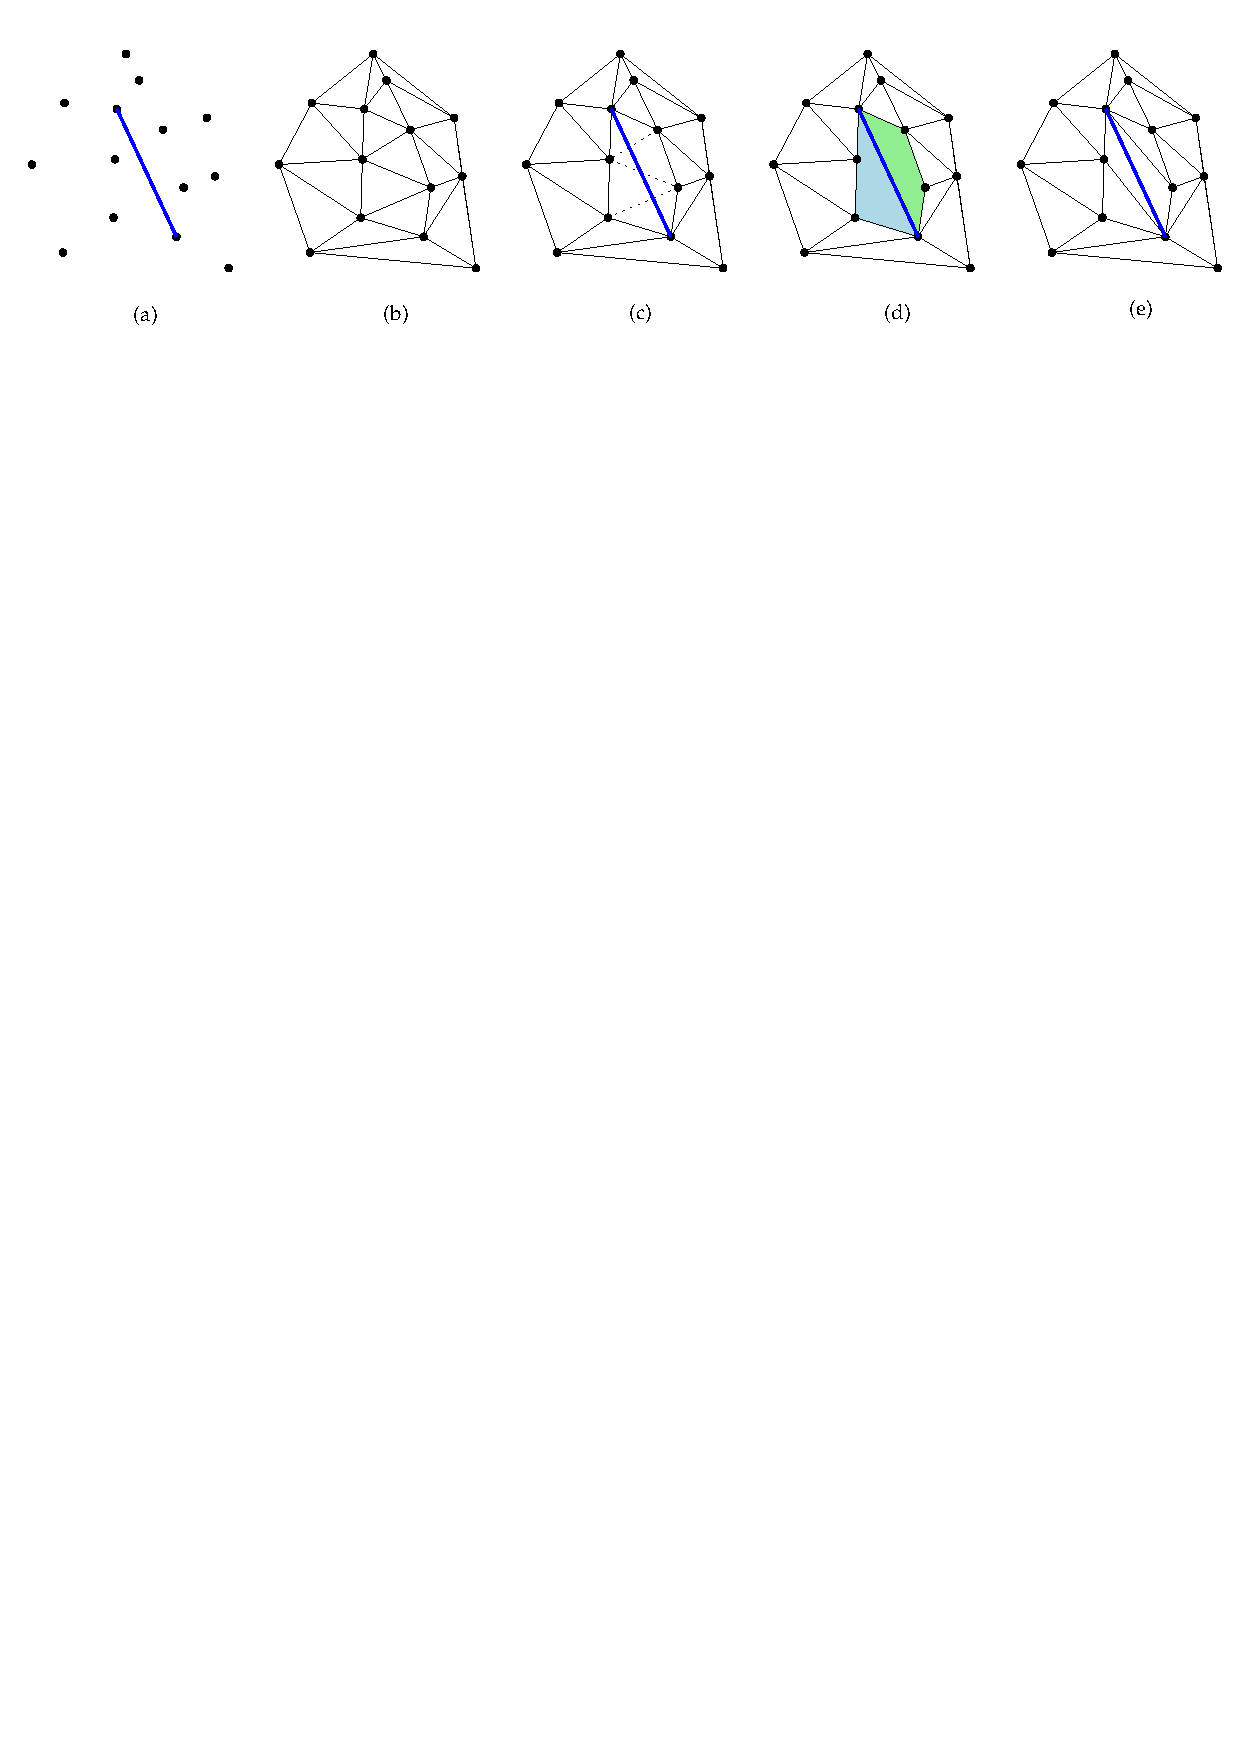
\includegraphics[width=0.95\linewidth]{figs/cdt_steps}
  \caption{Steps to construct a ConsDT.}%
\label{fig:cdt_steps}
\end{figure*}
\begin{enumerate}
  \item construct DT($S^p$), where $S^p$ is the set containing all the points in $S$ and the end points of the line segments (Figure~\ref{fig:cdt_steps}b)
  \item insert each line segment, each insertion will remove edges from DT($S^p$). In Figure~\ref{fig:cdt_steps}c 3 edges are removed.
  \item this creates 2 polygons that need to be retriangulated, in Figure~\ref{fig:cdt_steps}d there is a blue and a green one.
  \item retriangulate each separately, the Delaunay criterion needs to be verified only for the vertices incident to the triangles incident to the hole/polygon.
\end{enumerate}

%

Observe that the ConsDT can be used to triangulate polygons with holes (see Figure~\ref{fig:cdt_dog}), it suffices to remove the triangle outside the exterior boundary, but inside the convex hull.
\begin{marginfigure}
  \centering
  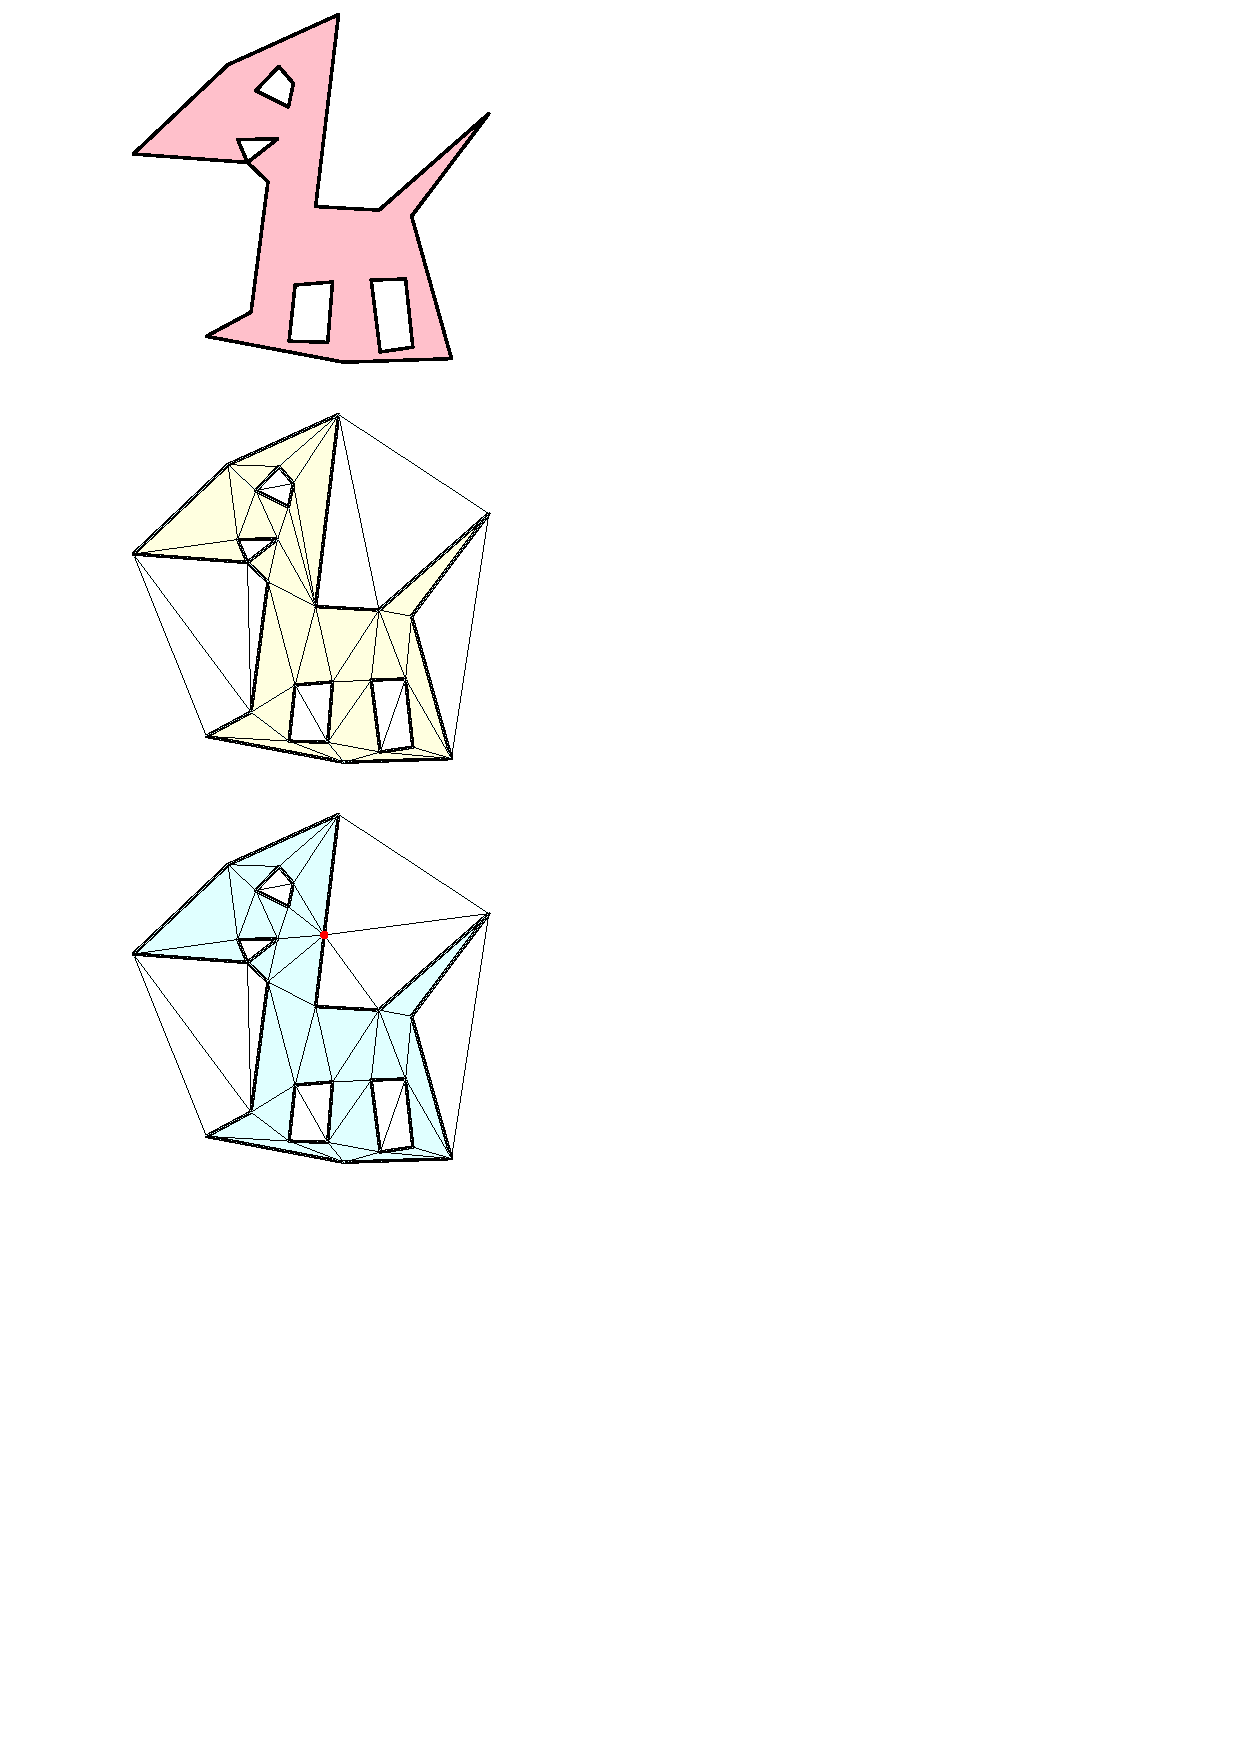
\includegraphics[width=0.8\linewidth]{figs/cdt_dog}
  \caption{\textbf{(top)} One polygon with 4 holes (interior rings). \textbf{(middle)} its ConsDT\@. \textbf{(bottom)} its ConfDT (the Steiner point added is in red).}%
\label{fig:cdt_dog}
\end{marginfigure}


%%%
%
\paragraph*{Conforming DT (ConfDT).}
A ConfDT adds new points to the input $S$ (called \emph{Steiner} points) to ensure that the input segments are present in the triangulation.% 
\index{Steiner point}\marginnote{Steiner point}
As Figures~\ref{fig:cdt_example} and~\ref{fig:cdt_dog} show, the input straight-line segments will be potentially split into several collinear segments. 
The Steiner points have to be carefully chosen (where to put them is beyond the scope of this course).

Observe that each triangle in a ConfDT respect the Delaunay criterion, but that more triangles are present. 
If 2 segments are nearly parallel, many points could be necessary (for $m$ segments, up to $m^2$ could be necessary).


%%%
%
\section{Notes and comments}%
\label{sec:notes}

The DT and the VD have been discovered, rediscovered and studied many times and in many different fields, see \citet{Okabe00} for a complete history.
The VD can be traced back to 1644, when Descartes used Voronoi-like structures in Part III of his \emph{Principia Philosophi\ae}. 
The VD was used by \citet{Dirichlet50} to study quadratic forms---this is why the VD is sometimes referred to as \emph{Dirichlet tessellation}---but was formalised and defined by \citet{Voronoi08}. 
The first use of the VD in a geographical context is due to \citet{Thiessen11}, who used it in climatology to better estimate the precipitation average around observations sites; the DT was formalised by \citet{Delaunay34}. 

For the construction of the DT, the incremental algorithm was first described by \citet{Lawson72-1}.
\citet{Guibas85} describe a divide-and-conquer algorithm, and \citet{Fortune87} a sweep-line one.

The local optimality of a DT, which implies globally optimality in the case of the DT, was proven by \citet{Delaunay34} himself.
The \emph{max-min angle optimality} of the DT was firstly observed by \citet{Sibson78}.
This paraboloic lifting was first observed by \citet{Brown79} (who used a spherical transformation), further described by \citet{Seidel82,Edelsbrunner86}. 

Instead of using a \emph{big triangle}, several will use an ``infinite point'' or a ``far-away point'', which is conceptually the same but numerically more stable (since the size of the big triangle does not need to be defined).
\citet{Liu05-1} explains the details.

The walking algorithm described, with a few modifications, can perform point location in $\mathcal{O}(n^{1/3}$).
The walking in the triangulation to locate the triangle containing a newly inserted point is not the fastest solution, \citet{Mucke99} and \citet{Devillers02} discuss alternatives that are optimal (\ie\ $\mathcal{O}(\log n)$).
However, they both note that optimal algorithms do not necessarily mean better results in practice because of the amount of preprocessing involved, the extra storage needed, and also because the optimal algorithms do not always consider the dynamic case, where points in the DT could be deleted. 

Several criteria for constructing data-dependent triangulations are discussed in \citet{Dyn90}. 
While these can be used, in practice it was proven that the Delaunay triangulation is still the triangulation that minimises the roughness of a surface~\citep{Wang01,Rippa90}

% TODO : complete this: uniqueness of the DT
% If the input points of the DT are not in general position, it is still possible to obtain a unique DT\@.
% This however means that 

\citet{Shewchuk97} shows that while the triangle-based data structure requires twice as much code as with the quad-edge (to store and construct a ConsDT), the result is that the code runs twice as fast and the memory requirement as about 2X less.
CGAL (\url{https://www.cgal.org/}), among many others, uses the triangle-based data structure.

Since a DT can be locally modified by adding one point (and not reconstructing the whole structure from scratch, see Figure~\ref{fig:insertion_deletion}), it is also possible to delete/remove one vertex from a DT with only local operations.
\citet{Mostafavi03} and \citet{Devillers09} describe algorithms.

The details of how the spatial interpolation methods generalise to 3D are given in \citet{Ledoux05}.

%%%
%
\section{Exercises}

\begin{enumerate}
  \item A DT has 32 triangles and we insert a new point $p$ that falls inside one of the triangles. If we insert and update the triangulation (for Delaunay criterion), what is the number of triangles?
  \item If a given vertex $v$ in a DT has 7 incident triangles, how many vertices will its dual polygon contain?
  \item A DT has 6 vertices, and 3 of these are forming the convex hull. How many triangles does the DT have?
  \item Assume you have 8 points located on a circle. Draw the DT and the VD of these 8 points.
  \item When inserting points in a DT (Algorithm~\ref{algo:insert1pt}), what happens if a new point is inserted directly on an edge? Line~2 states that the triangle is split into 3 new triangles, does it still hold?
  \item Given the input formed of elevation points and breaklines below (both projected to the $xy$-plane), draw both the constrained and conforming Delaunay triangulation (an approximation is fine).
  \\ \\
  \centering{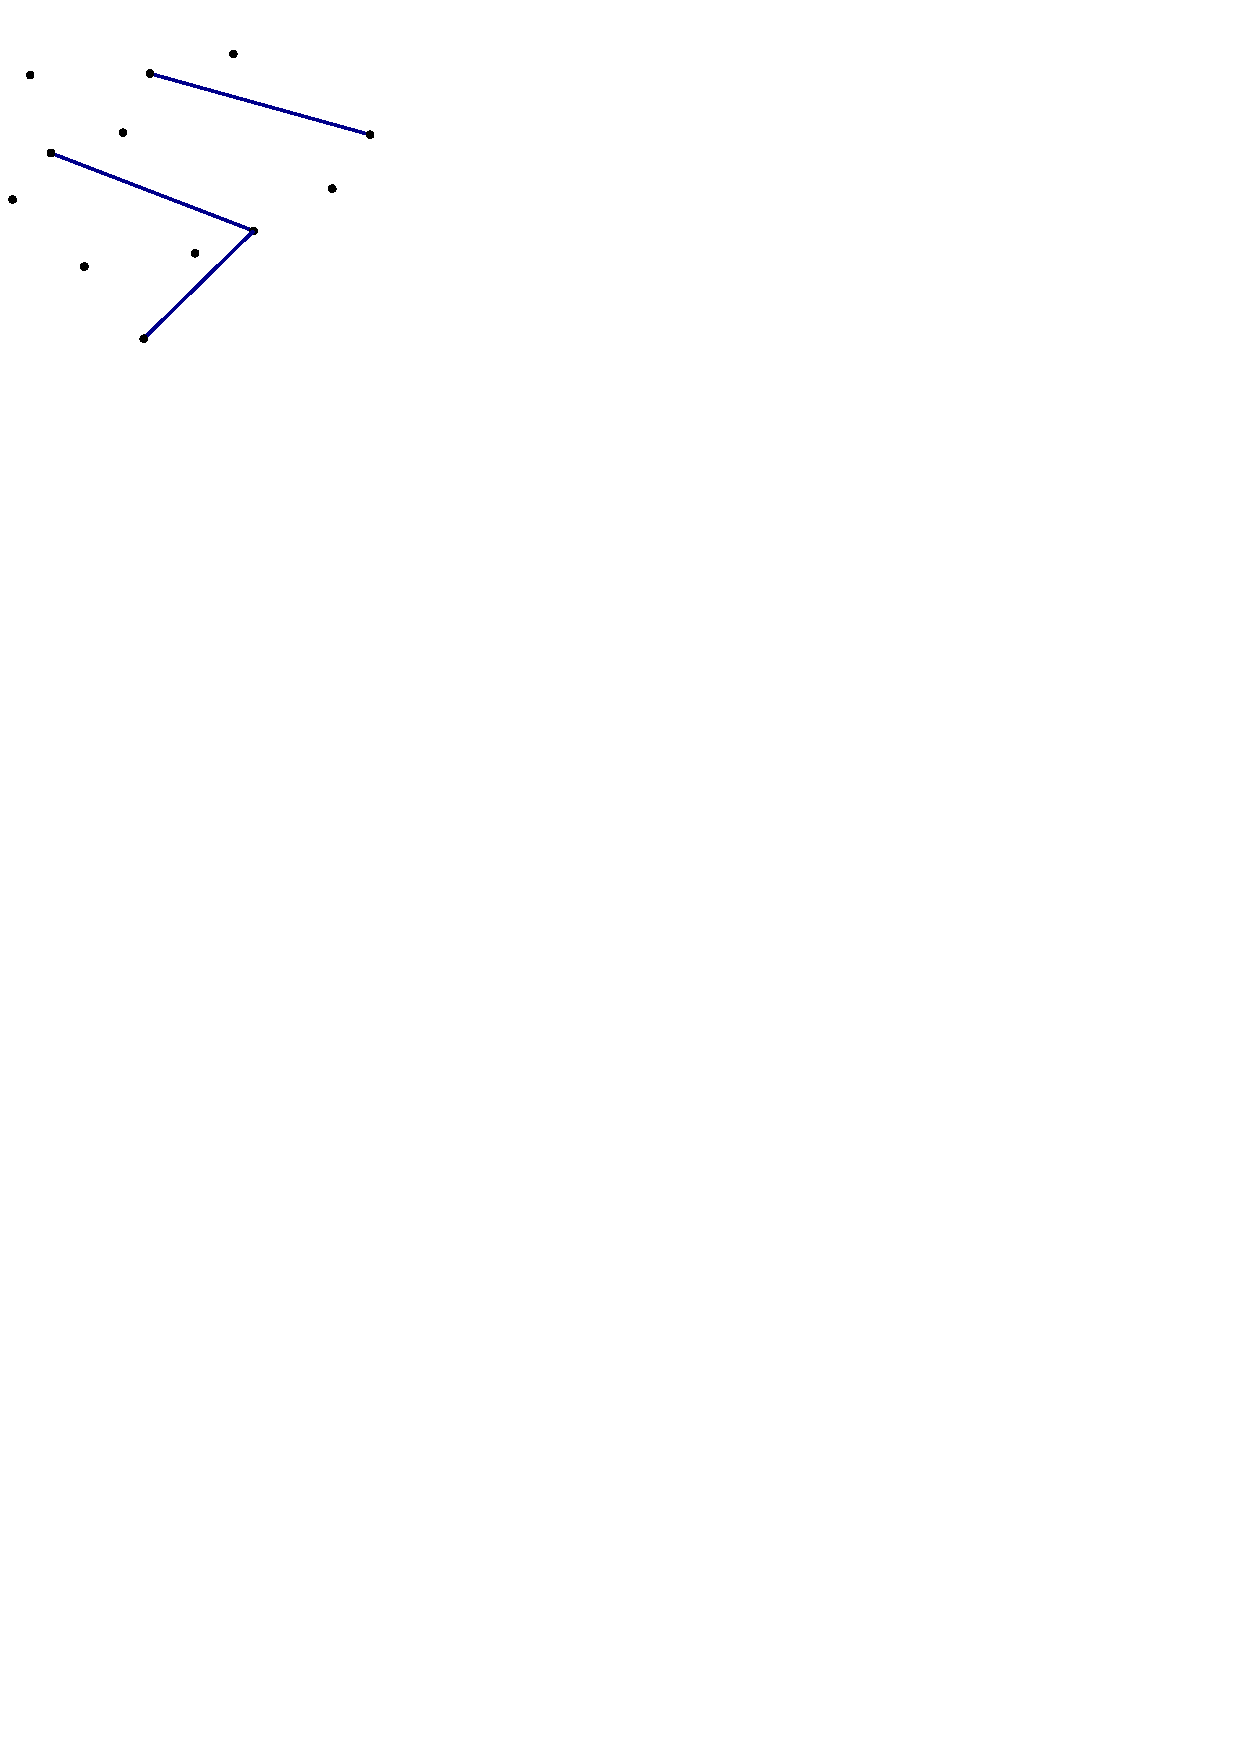
\includegraphics[width=0.95\linewidth]{figs/cdt_exercise}}
\end{enumerate}
